% !TeX program = xelatex
% Overleaf: main.tex + XeLaTeX. Collaboration draft; official cover is not supplied.
\documentclass[UTF8,a4paper,zihao=-4,fontset=fandol]{ctexart}
\usepackage[margin=22mm]{geometry}
\usepackage{amsmath,amssymb,graphicx,enumitem}
\usepackage[hidelinks]{hyperref}
\usepackage{caption}
\captionsetup{font=normalsize,labelsep=quad}
\ctexset{section={name={第,章},number=\chinese{section},format=\zihao{4}\heiti\centering},
subsection={number=\arabic{section}.\arabic{subsection},format=\zihao{-4}\heiti}}
\numberwithin{equation}{section}
\numberwithin{figure}{section}
\numberwithin{table}{section}
\renewcommand{\theequation}{\arabic{section}.\arabic{equation}}
\renewcommand{\thefigure}{\arabic{section}-\arabic{figure}}
\renewcommand{\thetable}{\arabic{section}-\arabic{table}}
\newcounter{alglinecount}
\newenvironment{algorithmblock}[1]{\par\medskip\noindent\begin{minipage}{\linewidth}
\hrule\vspace{5pt}\textbf{#1}\par\vspace{4pt}\hrule\vspace{5pt}\normalsize
\setcounter{alglinecount}{0}}{\par\vspace{5pt}\hrule\end{minipage}\par\medskip}
\newcommand{\alginput}[1]{\noindent\textbf{输入：}#1\par}
\newcommand{\algoutput}[1]{\noindent\textbf{输出：}#1\par\vspace{3pt}}
\newcommand{\algline}[2][0]{\stepcounter{alglinecount}\par\noindent
\hangindent=2em\hangafter=1\makebox[2em][l]{\arabic{alglinecount}.}\hspace*{#1em}#2\par}

\usepackage{longtable}
\linespread{1}
\pagestyle{plain}
\setlength{\parindent}{2em}
\begin{document}
\begin{center}
{\zihao{3}\heiti 通用神经网络处理器的结构感知切图与分层调度模型}\par\medskip
{\heiti 摘要}
\end{center}
多核神经网络处理器的执行效率受计算依赖、共享带宽与核内存储共同限制。针对三种逐层增加同步和缓存能力的运行场景，本文在保持原图语义与附件调度规则的条件下，建立以完工时间为主、兼顾额外搬运的切图与调度方法。

首先，将张量--操作二部图投影为操作依赖图，提取弱连通分量、层宽、双管道工作量与共享输入。对于无核间缓存同步的场景，采用完整分量装箱与结构切分相结合的有限构造，以任务工作量和依赖估计筛选方案，并对优先候选进行有限重排与合并。具备硬件同步后，将通信边界转为核心边界，以张量生命周期估计核内驻留风险，在同核复用与计算均衡之间选择。对于共享只读 FIFO Cache，进一步建立 DDR、L2 双带宽池事件模型，描述发射查询、完成插入与淘汰，并用核内换出估计修正候选时间。

冻结算法分别从原始输入独立生成方案，再由附件程序验收。100 图五核平均加速比分别为 3.8311、3.9522 和 4.1939。第二问的平均额外搬运较第一问减少 36.17\%；第三问固定同一方案开启 L2 后，平均耗时缩短 2.976\%，平均字节命中率为 26.45\%。三问已测正式方案均通过执行验收。独立新图检验同时发现第二问对输入表示和部分分层结构不够稳定，说明冷启动与有效的结构分析仍需配合独立性能验证。

本文通过有限结构构造和逐层细化的资源模型控制方案生成成本，用逐图对照区分通信减少、调度改变与缓存开关的效果。该方法在给定数据上兼顾求解速度与多核收益，后续改进重点为驻留时序近似和未见结构下的候选选择。

\textbf{关键词：}计算图切分；多核调度；张量生命周期；FIFO Cache；事件模型

\clearpage
\section{问题重述}

\subsection{计算图在多核处理器上的执行任务}
神经网络处理器的并行计算能力只有在数据及时到达、核内空间足够且任务依赖得到满足时才能发挥。矩阵与向量操作可以分配到不同核心，也可以在同一核心的不同管道上重叠执行；张量的搬入、搬出与临时驻留则占用另一组资源。神经网络加速器架构研究将计算组织和数据流组织视为密切相关的设计问题\cite{Chen2022}。本题将这种耦合具体化为给定硬件配置下的计算图切分、核心分配与子图排序问题。

题目提供 100 个计算图以及固定的核内调度、多核模拟程序。原图由张量节点与操作节点构成，边表示数据依赖；张量大小、所在存储层、操作周期及计算管道均已给定。求解者需要将非搬运操作划入若干子图，再为各核心安排子图执行序列。输出接口只有操作到子图的映射和每核子图序列，实际指令时刻、缓存换入换出以及共享带宽分配由附件机制产生\cite{Problem2026}。

切图同时改变了三个量：能够并行执行的计算工作量、跨任务或跨核心的数据传递量，以及张量在核内占用空间的时间。子图过大容易集中负载，子图过小又会增加边界搬运和同步。因而，问题的关键在于识别哪些依赖适合保留在核内，哪些计算区域值得以通信代价换取并行执行。

\subsection{三种场景的具体要求}
问题一采用场景 A：每个子图形成独立 Task，Task 之间不能直接延续核内缓存状态。即使两个子图位于同一核心，边界数据仍须经 DDR 传递；跨核依赖还具有固定等待开销。需要在这种机制下安排切图与任务顺序，尽量缩短系统完工时间并减少额外搬运。

问题二采用场景 B：同一核心的全部子图合并为一个 Task，同核生产与消费可以复用 L1/UB 中的数据。跨核依赖通过搬出、硬件同步和搬入建立联系。合并扩大了数据复用范围，也延长了部分张量的驻留，因此分核时需要兼顾通信内化、负载均衡与缓存压力。

问题三在场景 B 上增加所有核心共享的 1 MiB 只读 FIFO Cache。读取发射时查询缓存，命中读取使用独立的 L2 带宽；完成读取后按附件规则尝试插入，容量不足时按先入先出次序淘汰。需要利用合法的切图与排序形成共享读取机会，并比较同一方案在关闭和开启 L2 时的性能。

三问均要求在 1--5 核配置下汇总加速效果，保存逐图完工时间、额外搬运量及可复现方案。第三问还需给出 Cache 命中情况。问题一、二的单核参照采用整图单核方案；第三问对该固定方案补充缓存开关比较，不进行单核方案搜索。

\section{问题分析与总体思路}

\subsection{并行收益为何受到数据流限制}
依赖图中的独立分支提供并行执行机会，但计算量均衡并不等于完成时间均衡。一个核心即使承担较少计算，也可能长时间等待前驱数据；多个核心同时搬入时，又会竞争同一 DDR 带宽池。将一条大张量依赖切开，既增加搬运工作量，也可能把原本连续的计算链变成跨核等待链。判断一个切分是否值得，需要把计算、依赖与通信放在同一时间尺度上比较。

弱连通分量给出了较自然的起点：不同分量之间不存在计算依赖，保持分量完整可以避免切断其内部生产--消费关系。然而，分量可能共同读取同一个外部输入，分量内部也可能超过核内缓存容量。因此，完整分量装箱减少的是由内部切分引入的边界代价，并不意味着总 DDR 流量为零。若最大分量占据大部分工作量，还必须考察其内部并行结构。

输入图的另一项差异来自计算管道。相同的操作周期总和可能对应不同的矩阵、向量工作量组成；若仅按总周期分核，两个核心可能分别拥堵在不同管道，或一个核心的单管道成为瓶颈。本文在分量和子图层面保留双管道负载，再通过通信与依赖估计比较可行划分。

\subsection{从任务边界到数据驻留和读取时序}
场景 A 中，切图边界直接决定 Task 边界，减少不必要边界有助于降低重复搬运。场景 B 中，同核子图可以连续复用数据，优化重点转向哪些操作应被安排在同一核心。把共享张量的消费者集中起来能够减少跨核读取，却也可能延迟张量的最后一次使用，使缓存长期被占用。本文以张量的首次出现和末次使用估计驻留区间，将容量压力引入候选排序。

只读 Cache 又增加了一项时间条件：第二次读取必须在首次读取完成之后、条目被淘汰之前发射，才能形成命中。共享输入很多并不足以说明收益大；如果各核同时发起首次读取，或共享张量很快被新条目挤出，潜在复用不会转化为带宽收益。第三问因而继承场景 B 的分核与驻留分析，并进一步展开读写请求的事件时序。

\begin{figure}[htbp]
\centering
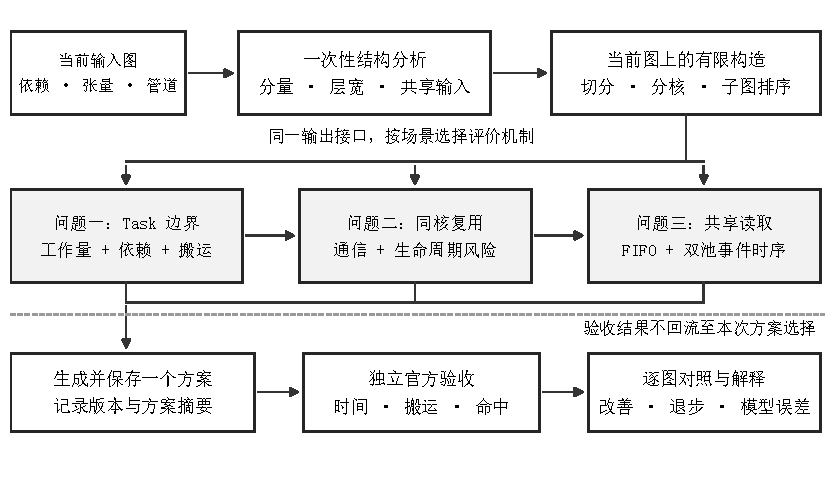
\includegraphics[width=\linewidth]{figures/fig2_1.pdf}
\caption{三问共用的决策过程及逐层增加的运行机制。输入结构在每个图上重新计算；实线连接求解所用信息，底部表示方案保存后的独立验收。图中节点为建模环节，不代表实际执行时间。}
\label{fig:overall}
\end{figure}

\subsection{已有方法的启发与本题的实现范围}
深度学习编译器研究强调图表示、调度和目标硬件之间的配合\cite{Liu2025}。经典最长作业优先分配与列表调度分别提供了负载分散和关键路径优先的构造思路\cite{Graham1969,Topcuoglu2002}。这些方法能够低成本产生初始方案，但本题的任务时间会随切图、缓存换出和共享带宽竞争变化，不能直接套用独立定长作业模型的性能界。

基于性能建模的调度研究说明，估计模型的用途在于把任务和资源信息转化为可比较的决策依据\cite{Yang2025}。本文采用有限种结构构造，并让统一模型对当前图产生的方案进行排序。候选是一次求解过程中的中间决策，最终接口仍接收一个图并输出一个方案。构造数量受到显式限制，避免把大部分时间用于反复调用耗时的完整模拟。

MAGIS 将图优化与调度中的延迟、内存开销联合考虑\cite{Chen2024}，Timeloop 用架构和数据流模型分析加速器的存储与执行代价\cite{Parashar2019}。本文从中吸收张量生命周期分析和资源服务量建模的思路，具体实现保持题目原计算图与固定硬件配置。既不进行算子融合、计算复制或重计算，也不引入题目未给出的张量分块与映射维度。

三个问题具有完工时间与额外搬运量两个评价方向。本文将完工时间置于主要位置，用搬运量和驻留风险修正时间代理或打破并列。当前算法采用确定性构造与评分选择，未执行非支配排序或种群进化；后文公式和伪代码均围绕这一实际求解过程展开。

\section{模型假设与符号说明}

\subsection{题设条件与估计假设}
张量大小、操作周期、数据依赖和存储位置以实际附件为准。计算图保持原语义，每个非 COPY 操作恰好执行一次；核心数、四条管道、缓存容量、同步延迟及带宽取题目配置。它们是约束模型的已知条件。

候选比较采用三项估计约定。第一，以当前图的计算工作量和依赖路径构造确定性的时间估计，不额外引入操作周期随机扰动。第二，问题一、二用任务或核心的汇总工作量近似资源拥堵，问题三将读写服务展开为事件；估计精度随模型层次增加，但不将任何一项代理量视为官方执行时间的恒等式。第三，核内驻留估计采用分析序列上的张量使用区间，实际空间复用及换出插入仍由固定执行机制确定。

这些约定使每次方案生成只依赖当前输入图、硬件配置和冻结参数。全局参数可以在开发阶段诊断、标定；正式生成方案时不读取历史答案或该图旧得分。已给定 100 图参与过开发，故全量成绩用于报告本题数据上的性能，独立输入测试另行列示。

\subsection{统一符号与计量单位}
原始图记为 $G=(T\cup O,E)$，非 COPY 操作集合为 $O_c$。本文用 $t$ 表示张量索引、$u,v$ 表示操作索引、$s$ 表示子图、$k$ 表示核心；物理时刻记为 $\theta$。张量大小统一用 byte，时间统一用 cycle，图中 MiB 按 $2^{20}$ byte 换算。

\begin{table}[htbp]
\centering
\caption{主要符号及其含义，局部辅助量在对应公式前定义}
\label{tab:notation}
\begin{tabular}{p{0.28\linewidth}p{0.59\linewidth}}
\hline
符号 & 定义与单位 \\
\hline
$s_t,c_u,p(u)$ & 张量字节数、操作周期、操作所属计算管道 \\
$G_c=(O_c,E_c)$ & 由原图生产--消费关系投影得到的操作依赖图 \\
$\mathcal C,C_j,K$ & 弱连通分量集合、第 $j$ 个分量及分量数 \\
$d_u,h,m_\ell$ & 操作拓扑深度、最大深度及第 $\ell$ 层操作数 \\
$N,k$ & 核心数与核心编号，$k=0,\ldots,N-1$ \\
$\mathcal S,\phi,a,\pi_k$ & 子图集合、操作归属、核心分配及核心 $k$ 的子图序列 \\
$P$ & 完整方案 $(\phi,a,\pi_0,\ldots,\pi_{N-1})$ \\
$W_j^q,L_k^q$ & 分量或核心在管道 $q\in\{M,V\}$ 上的工作量，cycle \\
$C_r,\beta,\beta_{\rm L2}$ & 存储容量 byte；DDR、L2 总带宽 byte/cycle \\
$T^{X}(P),D^{X}(P)$ & 场景 $X$ 中实际完工时间、官方额外搬运量 \\
$\widehat T,\widehat B,J$ & 时间估计、字节数估计及候选评分 \\
$T_{i,1},\overline S_N$ & 第 $i$ 图的整图单核参照、$N$ 核逐图加速比均值 \\
\hline
\end{tabular}
\end{table}

带帽变量来自求解模型，无帽的执行时间和搬运结果来自方案冻结后的验收。$\phi$ 与 $\pi_k$ 对应提交字段；$a$ 可由子图在核心序列中的位置恢复。该区分使建模解释、求解输出与结果统计保持一致。

\input{sections/04.tex}
\section{数据预处理与结构特征分析}

\subsection{原始字段到计算依赖的转换}
本章的数据预处理与结构特征分析使用 OpenAI GPT-6（模型标识：gpt-6-astra；发布日期：2026 年 9 月 3 日）辅助梳理分析思路和结果表述\cite{AIGPT6}。表中统计量由项目脚本根据 100 张原始计算图计算；队伍核对数据来源、计算过程与解释。工具使用范围及人工复核责任见附录。

预处理按节点类型解析张量、计算操作和搬运操作，保留原始标识与字段。原始图在既有独立验收中通过附件的字段和图结构校验；本轮逐一核对 100 图 SHA256 与结构表记录一致。描述性统计读取原始字段，张量大小与操作周期均不重估，以便后续结果可追溯到同一输入。正式求解入口尚未覆盖的非法输入检查在第九章单列，不将离线数据核查等同于程序具备全部输入防护。

从操作集合中取出非 COPY 操作 $O_c$，经张量连接的生产与消费关系投影为
\begin{equation}
G_c=(O_c,E_c),\qquad
E_c=\{(u,v)\in O_c^2:\exists t\in T,\ (u,t),(t,v)\in E\}.
\label{eq:q1-opgraph}
\end{equation}
投影图用于判断操作先后及计算区域。张量标识、大小、生产者和消费者继续保存在索引表中，因此同一张量被多个操作消费时，可以按其实际共享关系计算搬运和驻留，而不把每条投影边都当作一份独立数据。原图中的 COPY 还用于识别输入读入与最终输出；投影不删除最终执行所需的搬运。

\subsection{面向调度的结构量}
对 $G_c$ 进行拓扑排序，并在其无向形式上提取弱连通分量 $\mathcal C=\{C_1,\ldots,C_K\}$。沿拓扑序计算深度与层宽，再累计各分量的双管道工作量：
\begin{equation}
\begin{aligned}
d_u&=1+\max_{v\in\operatorname{pred}(u)}d_v,\quad h=\max_u d_u,\\
m_\ell&=|\{u:d_u=\ell\}|,\qquad
W_j^q=\sum_{u\in C_j,\ p(u)=q}c_u,\quad q\in\{M,V\}.
\end{aligned}
\label{eq:q1-features}
\end{equation}
无前驱操作的深度为 1。入度大于 1 标识汇合位置，出度大于 1 标识分支位置。总工作量 $W=\sum_u c_u$ 与计算关键路径长度 $L$ 由
\begin{equation}
\lambda_u=c_u+\max_{v\in\operatorname{pred}(u)}\lambda_v,\qquad
L=\max_u\lambda_u,\qquad \rho=W/L
\label{eq:span}
\end{equation}
得到，空前驱的最大值取零。$\rho$ 描述忽略通信和资源竞争后的工作量与路径长度之比，用于观察潜在并行结构；它不等于本题实际可取得的加速比。

还统计最大分量操作数占比与向量工作量占比：
\[q_{\max}=\frac{\max_j|C_j|}{|O_c|},\qquad q_V=\frac{\sum_{p(u)=V}c_u}{W}.\]
此外，统计具有两个及以上非 COPY 消费者的外部输入张量数。$q_{\max}$ 按操作个数计算，与最大分量的周期占比不同。对于操作周期差异明显的图，后续装箱直接使用 $W_j^M,W_j^V$，不以节点个数代替负载。

\begin{table}[htbp]
\centering
\caption{100 个原始计算图的描述性统计}
\label{tab:inputstats}
\begin{tabular}{lrrr}
\hline
统计量 & 最小值 & 中位数 & 最大值 \\
\hline
非 COPY 操作数 & 552 & 3720.5 & 35705 \\
操作依赖边数 & 400 & 4017 & 38493 \\
弱连通分量数 $K$ & 1 & 39.5 & 2666 \\
拓扑深度 $h$ & 3 & 47.5 & 2440 \\
计算工作量 $W$/cycle & 23052 & 509952 & 61275840 \\
计算关键路径 $L$/cycle & 400 & 6140 & 863040 \\
工作量与路径比 $\rho$ & 3.42 & 43.13 & 6258.78 \\
\hline
\end{tabular}
\end{table}

\begin{figure}[htbp]
\centering
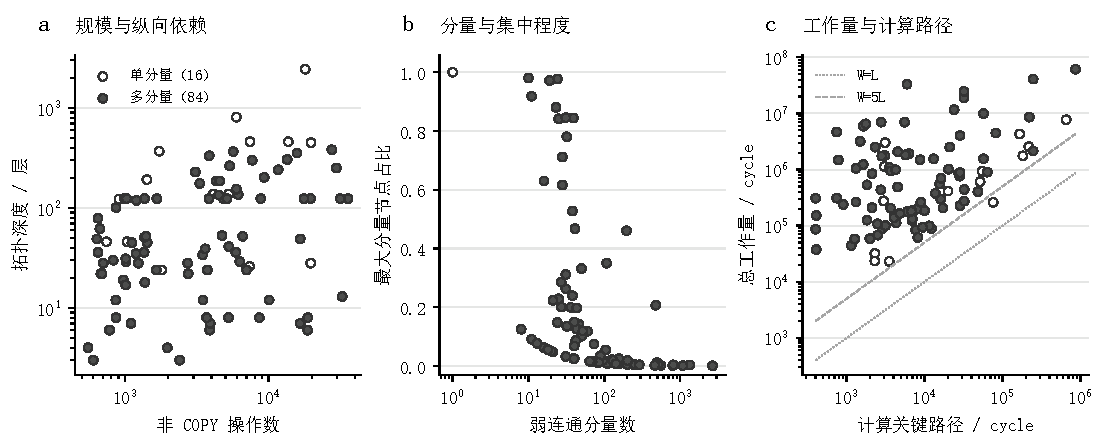
\includegraphics[width=\linewidth]{figures/fig5_1.pdf}
\caption{100 图的结构与工作量差异，每个点代表一张原始图。a 操作规模与拓扑深度；b 分量数与最大分量节点占比；c 计算关键路径与总工作量，参考线表示 $W=L$ 和 $W=5L$。空心、实心符号区分单分量和多分量图。对数坐标用于展示数量级跨度，不改变特征计算。}
\label{fig:inputstats}
\end{figure}

\subsection{特征如何进入三问决策}
84 个图具有多个弱连通分量，且其分量数均不少于 5；另有 16 个图只有一个分量。前一类通常提供直接分配独立计算块的机会，后一类若只保持分量完整，将无法利用多个核心。最大分量节点占比的中位数约为 0.122，也存在接近 1 的图，说明“分量很多”和“负载容易均衡”仍需分别判断。

共有 97 个图包含被多个计算操作消费的外部输入。这些输入是问题三共享读取的潜在来源，但它们也可能在同一核心内部完成复用，或因请求同时到达而无法命中 L2。此处统计仅用于识别可利用的数据关系；实际收益由第八章的事件模型及配对实验判断。

\begin{table}[htbp]
\centering
\caption{预处理特征与后续决策的对应关系}
\label{tab:featureuse}
\begin{tabular}{p{0.24\linewidth}p{0.29\linewidth}p{0.36\linewidth}}
\hline
原图信息 & 计算量 & 对应建模作用 \\
\hline
生产--消费依赖 & 分量、拓扑序、分支与汇合 & 第六章保留完整分量或选择内部切分位置 \\
操作周期与管道 & $W_j^M,W_j^V$ & 三问共用的双管道负载分配 \\
深度和层宽 & $h,m_\ell$、结构层间距 & 确定深度带尺度与层宽收缩边界 \\
张量大小与消费者 & 边界字节、跨核消费集合 & 第六、七章的搬运估计与同核复用 \\
存储位置与使用序列 & 活跃区间、峰值、下一次使用 & 第七、八章的 L1/UB 风险与换出估计 \\
共享输入与访问事件 & 读取先后、FIFO 驻留窗口 & 第八章的读路径选择与缓存收益解释 \\
\hline
\end{tabular}
\end{table}

结构特征在输入到达时重新提取。算法不把 100 图的均值、分位数或用例编号作为类别阈值；表~\ref{tab:inputstats} 和图~\ref{fig:inputstats} 用来解释输入差异，实际构造尺度由各图自身的深度、工作量及分支位置计算。这样的分工使数据分析与算法机理相互连接，同时保留了对新图进行结构分析的接口。

\section{问题一：基于拓扑结构的切图与任务调度}

\subsection{由独立分量到内部切分的决策}
场景 A 将子图边界转化为独立 Task 边界。第五章识别出的弱连通分量可以作为初始分配单位，在不切断内部依赖的条件下分散计算；单分量或负载高度集中的输入，则需要从内部切分获得并行机会。两类方案的取舍取决于新增并行工作量能否覆盖边界搬运和固定等待。

本问沿用式~\eqref{eq:q1-opgraph} 的操作依赖图和式~\eqref{eq:q1-features} 的双管道工作量。先以完整分量装箱得到低边界代价方案，再从分支、汇合及层宽变化构造少量替代划分；时间估计负责比较这些结构选择，局部任务重排与合并用于处理优先候选中的等待和冗余边界。

\subsection{场景 A 的约束与时间估计}
对给定核心数 $N\in\{2,3,4,5\}$，沿用子图映射 $\phi:O_c\to\mathcal S$，核心分配为 $a:\mathcal S\to\{0,\ldots,N-1\}$，核心 $k$ 的子图执行序列为 $\pi_k$。子图编号为非负整数；每个非 COPY 操作必须且只能分配到一个子图，每个子图必须且只能在一个核心序列中出现一次。子图依赖图以及加入同核先后关系后的联合图均须无环。输出采用附件规定的 \texttt{node\_to\_subgraph} 和 \texttt{core\_schedules} 两个字段。

以系统完工时间为主要优化目标，同时考虑新增 DDR 搬运量。根据固定配置，同核相邻 Task 的等待时间为 $\delta_{\rm same}=100$ cycle，跨核前驱 Task 的等待时间为 $\delta_{\rm cross}=1000$ cycle；各核心共同使用带宽 $\beta=60$ byte/cycle 的 DDR。L1 和 UB 的容量分别为 524288 byte 和 131072 byte。增加核心数不会增加 DDR 总带宽，同核 Task 切换也不能保留前一 Task 的缓存数据。

为在有限时间内比较候选，采用计算工作量、边界字节数和任务依赖共同构成时间估计。设 $I_s$、$U_s$ 为 Task $s$ 需要从 DDR 读入和写回 DDR 的张量集合，同一 Task 内按张量去重，则
\begin{equation}
\widehat B_A=\sum_{s\in\mathcal S}\left(\sum_{t\in I_s}s_t+\sum_{t\in U_s}s_t\right),\qquad
\widehat d_s=\max\left\{W_s^M,W_s^V,
\frac{\sum_{t\in I_s}s_t+\sum_{t\in U_s}s_t}{\beta}\right\}.
\label{eq:q1-duration}
\end{equation}
这里 $W_s^q$ 按式~\eqref{eq:q1-features} 对 Task 内操作重新求和。两条计算管道和搬运可以重叠执行，故采用三类工作量所需时间的最大值估计 Task 时长。$\widehat B_A$ 记录任务边界的读写量；缓存不足产生的换入换出尚未进入该估计，后续官方验收将保留这一部分实际开销。

在子图依赖图中加入同核相邻 Task 的顺序边，记得到的前驱集合为 $P^\pi(s)$。沿该图的拓扑序递推：
\begin{equation}
\begin{aligned}
\widehat f_s&=\widehat d_s+\max_{u\in P^\pi(s)}(\widehat f_u+\delta_{us}),\\
\widehat T_A&=\max\left\{\max_s\widehat f_s,\frac{\widehat B_A}{\beta}\right\},\qquad
\delta_{us}=\begin{cases}
\delta_{\rm cross},&a(u)\ne a(s),\\
\delta_{\rm same},&u\text{ 为 }s\text{ 的同核紧邻前项},\\
0,&\text{其余同核依赖}.
\end{cases}
\end{aligned}
\label{eq:q1-time}
\end{equation}
空前驱集合的最大值取 0。任务的预计启动时刻取决于前驱完成和同核队列的末端，两类约束在同一递推中合并。全局项 $\widehat B_A/\beta$ 则避免将共享 DDR 当作各核独享资源。该模型省略了逐个 COPY 请求的动态带宽竞争，适合对有限候选作快速排序；结果部分使用方案冻结后获得的官方完工时间与搬运量。

\subsection{分量装箱与结构切分}
首先将弱连通分量作为完整物品分配。按 $\max(W_j^M,W_j^V)$ 从大到小处理分量，设核心 $k$ 已分配的管道负载为 $(L_k^M,L_k^V)$，则将当前分量放入
\begin{equation}
k^*=\arg\min_k
\left(\max_{q\in\{M,V\}}(L_k^q+W_j^q),\ L_k^M+L_k^V,\ k\right).
\label{eq:q1-packing}
\end{equation}
括号内按字典序比较，选定后更新两条管道负载。同核分量合并为一个子图，空核保留空序列。该规则采用最长工作量优先分配思想\cite{Graham1969}，并用双管道负载替代单一处理时间。共享 DDR 和缓存使本题不再满足经典独立作业调度模型，因而不直接援引其近似比作为本算法的性能保证。

完整分配保留了每个分量内部的生产--消费关系，分量之间也没有计算依赖，因而能够减少中间张量的跨核搬运。共享输入仍可能被多个核心分别读取，核内空间不足仍会触发换入换出。若一个分量集中了大部分计算量，完整分配还会使负载集中在单核上。内部切分候选主要用于处理这一类并行度受限的输入。

内部切分围绕三类结构展开。第一类保留首次汇合前的独立分支，或按照末端消费者对分支归组；第二类利用拓扑层宽的收缩与扩张确定阶段边界；第三类按照深度带与源端、末端可达关系划分。在深度带构造中，候选边界附近按跨层张量字节数选择切分位置，以减少将大张量切到不同 Task 的情况。上述构造均保持原操作和依赖，不拆分操作，也不复制计算。

基础深度带宽由当前图的深度 $h$、总计算量 $W=\sum_{u\in O_c}c_u$ 和核心数确定：
\begin{equation}
w_0=\max\left\{2,\left\lceil\frac{N\delta_{\rm cross}h}{\max(1,W)}\right\rceil,
\left\lceil\frac{Nh}{256}\right\rceil\right\}.
\label{eq:q1-band}
\end{equation}
算法考察 $w_0,2w_0,4w_0$ 三种粒度。前一项避免过细切分，第二项使计算相对等待开销较小时倾向于更粗的 Task；第三项是固定的搜索规模控制规则，256 不是题目的硬件常数。此外，还保留减少活跃核心数的分量分配候选，以应对并行计算收益不足以抵消 DDR 争用的情形。

\subsection{任务列表调度与有限合并}
各结构候选先经过覆盖性、无环性检查和方案去重，再由式~\eqref{eq:q1-time} 排序。仅对排名靠前的至多三个候选进行任务调度与合并调整，以控制额外搜索量。

任务重排采用“就绪任务优先级--最早完成核心”的列表调度思想\cite{Topcuoglu2002}。先自后向前计算
\begin{equation}
r_s=\widehat d_s+\max_{v\in\operatorname{succ}(s)}(\delta_{\rm same}+r_v).
\label{eq:q1-rank}
\end{equation}
每次从全部已分配前驱的就绪 Task 中选取 $r_s$ 最大者，比较其放到各核心后的预计完成时刻。设 $F_k$ 是核心 $k$ 已排任务的末端时间，则
\begin{equation}
\operatorname{EFT}(s,k)=\widehat d_s+
\max\left\{F_k+\delta_{\rm same}\mathbf1[\pi_k\ne\varnothing],
\max_{u\in\operatorname{pred}(s)}
\big(\widehat f_u+\delta_{\rm cross}\mathbf1[a(u)\ne k]\big)\right\}.
\label{eq:q1-eft}
\end{equation}
优先选择 EFT 最小的核心，并列时依次选择已排 Task 数较少、编号较小的核心。式~\eqref{eq:q1-rank} 中的固定等待项只用于任务优先级；核心选择时则按式~\eqref{eq:q1-eft} 区分同核与跨核等待。这里采用尾部追加排布，没有执行 HEFT 的空闲区间插入步骤。

合并调整只考虑同核相邻、且在 Task 拓扑序中也相邻的任务对。每轮按共享张量字节数选取至多八对，分别计算收缩后的方案；联合依赖图有环的方案被剔除，在其余方案中选取能够降低 $\widehat T_A$ 的一项，最多执行两轮。任务重排与合并均从原结构候选独立出发，二者不串接。最终按预计时间、边界字节数和固定方案哈希依次比较；当完整分量方案与最优估计相差不超过 1\% 时，保留完整分量方案。该阈值降低了选择结果对微小估计误差的敏感性。

\begin{algorithmblock}{算法 6-1\quad 基于输入拓扑的切图与任务调度}
\alginput{当前计算图 $G$，核心数 $N$，带宽 $\beta$，等待参数 $\delta_{\rm same},\delta_{\rm cross}$。}
\algoutput{子图映射 $\phi$ 与每核子图序列 $\pi_0,\ldots,\pi_{N-1}$。}
\algline{读取张量、操作与边；提取非 COPY 操作集 $O_c$，保留原始数据。}
\algline{按生产--消费关系构建 $G_c$；计算拓扑序与节点深度 $d_u$。}
\algline{提取弱连通分量、层宽、分支及汇合位置，统计双管道工作量与张量字节数。}
\algline{按式~\eqref{eq:q1-packing} 构造完整分量方案 $P_0$，初始化待检验集合 $\mathcal B\leftarrow\{P_0\}$。}
\algline{将首次汇合、末端分支与较少活跃核心数的分量装箱候选加入 $\mathcal B$。}
\algline{按式~\eqref{eq:q1-band} 计算 $w_0$。}
\algline{\textbf{for} $w\in\{w_0,2w_0,4w_0\}$ \textbf{do}}
\algline[1]{构造数据感知深度带、分支汇合、层宽谷和末端可达归组候选，加入 $\mathcal B$。}
\algline{\textbf{end for}；将宽度为 $w_0$ 的源端可达归组候选加入 $\mathcal B$。}
\algline{逐项检验 $\mathcal B$，将覆盖完整、联合图无环且不重复的方案组成 $\mathcal P$；记录拒绝原因。}
\algline{按式~\eqref{eq:q1-duration}--\eqref{eq:q1-time} 评价 $\mathcal P$；按时间、字节数截取至多三个原始候选。}
\algline{\textbf{for} 所选方案中的每个 $P$ \textbf{do}}
\algline[1]{从 $P$ 分别生成就绪列表重排方案与至多两轮的相邻任务合并方案。}
\algline[1]{重新检查合法性，计算时间估计，将不同的合法方案加入 $\mathcal P$。}
\algline{\textbf{end for}}
\algline{取 $\widehat T_A$ 最小的 $P^*$；时间并列时比较边界字节数与固定方案哈希。}
\algline{若 $\widehat T_A(P_0)\le1.01\widehat T_A(P^*)$，令 $P^*\leftarrow P_0$。}
\algline{\textbf{return} $P^*$ 的 \texttt{node\_to\_subgraph} 与 \texttt{core\_schedules}。}
\end{algorithmblock}

\subsection{求解结果与分析}
算法对每个图、每种核数分别从原始输入生成方案。所有全局参数在正式运行前固定，生成过程中不读取历史方案和逐图得分，也不调用官方评估器。方案保存后，再使用未修改的附件程序完成 100 个图、2--5 核共 400 组验收，全部通过。

设第 $i$ 个图在 $N$ 核下的官方完工时间为 $T_{i,N}$，按题目规定采用的单核整图时间为 $T_{i,1}$。统计采用逐图加速比的算术平均：
\begin{equation}
S_{i,N}=\frac{T_{i,1}}{T_{i,N}},\qquad
\overline S_N=\frac1{100}\sum_{i=1}^{100}S_{i,N}.
\label{eq:q1-speedup}
\end{equation}
单核加速比按定义置为 1，不另行进行单核搜索。表~\ref{tab:q1-result} 给出全部用例的汇总；额外搬运采用官方 \texttt{added\_copy\_bytes} 字段，并按 $1\,\mathrm{MiB}=2^{20}$ byte 换算。

\begin{table}[htbp]
\centering
\caption{问题一的全量求解结果}
\label{tab:q1-result}
\begin{tabular}{crrr}
\hline
核心数 & 平均加速比 & 加速比中位数 & 平均额外搬运 / MiB \\
\hline
2 & 1.8648 & 1.9583 & 13.848 \\
3 & 2.6016 & 2.7753 & 14.514 \\
4 & 3.2650 & 3.5074 & 15.557 \\
5 & 3.8311 & 4.0428 & 15.285 \\
\hline
\end{tabular}
\end{table}

\begin{figure}[htbp]
\centering
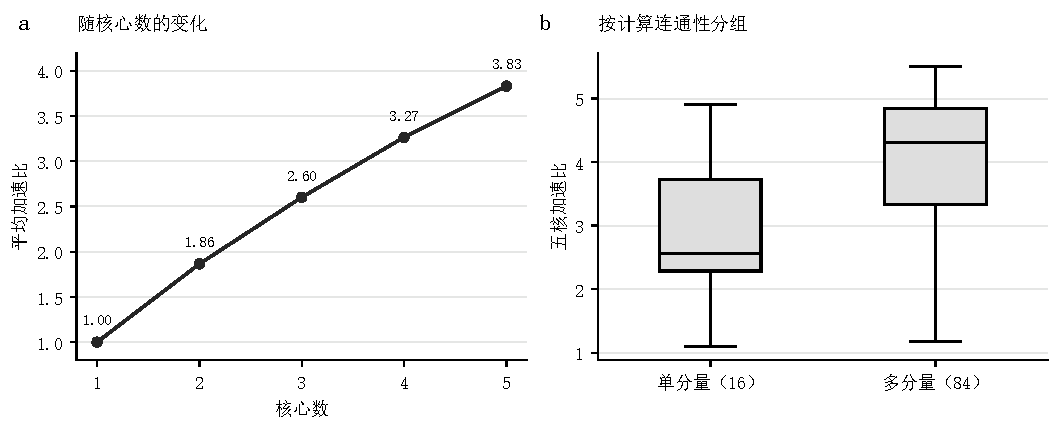
\includegraphics[width=\linewidth]{figures/fig6_1.pdf}
\caption{问题一的加速比结果。左图为每种核数下 100 图的算术平均，单核值按定义为 1；右图为五核下按弱连通分量数分组的分布。箱体表示四分位区间，中线为中位数，须延至 1.5 倍四分位距内的最远观测，点为其外观测。}
\label{fig:q1-result}
\end{figure}

五核平均加速比为 3.8311。多分量图的五核平均值为 4.0041，单分量图为 2.9228，表明输入结构对可利用的并行性有明显影响。多分量允许在较少新增依赖的条件下分配负载；单分量则通常需要在并行化与边界代价之间作出取舍。这一差异与独立分量提供可直接分配计算块的机制一致，分组内仍存在较大离散，故还需观察逐图对照。

与仅采用完整分量装箱的同批五核方案相比，增加结构切分与有限调度调整后，38 个图耗时下降、2 个图上升、60 个图不变。改进集中在完整分量分配以外的候选被选中后取得收益的输入上，少数退步反映了代理排序与实际执行的差异。五核平均额外搬运中，缓存换入换出占 7.423 MiB；任务边界之外的核内空间开销已达到不可忽略的规模。场景 B 延长了同核张量的可驻留范围，对这部分开销需要进一步建模。

\begin{figure}[htbp]
\centering
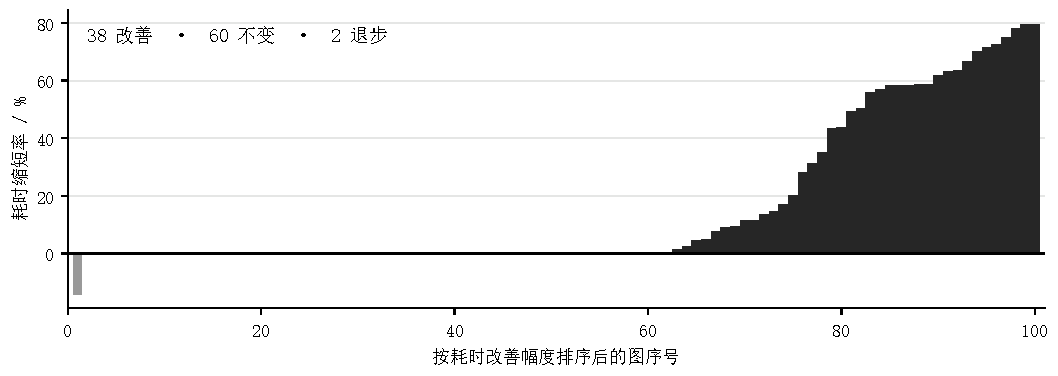
\includegraphics[width=\linewidth]{figures/fig6_2.pdf}
\caption{五核下相对于完整分量装箱的逐图耗时变化。横轴为全部 100 图按改善幅度排序后的序号，纵轴为 $100(1-T_A/T_{\rm component})$；零线以上表示扩展结构候选后的最终方案更快。该对照在同一场景 A 下验收，用于观察候选扩展及选择的综合作用。}
\label{fig:q1-comparator}
\end{figure}

图~\ref{fig:q1-comparator} 保留全部未改善和退步的用例。大量零变化说明在这些图上，低边界代价的分量分配已经足以被最终规则保留；正向尾部反映了内部切分和任务顺序调整的价值。两个退步用例则提示，有限候选中的代理最优仍可能低于分量对照的实际表现，继续增加构造数量并不能自动修复这一排序误差。

\input{sections/07.tex}
\input{sections/08.tex}
\section{综合评价与适用范围}

\subsection{三问的收益与计算代价}
三种模型围绕同一决策接口逐步细化：问题一比较保留分量与释放内部并行的代价，问题二引入同核数据驻留，问题三展开共享读取的事件顺序。对应五核平均加速比分别为 3.8311、3.9522 和 4.1939。三者使用相同整图单核参照，平均值都先计算逐图比值再汇总；这些数字反映本题 100 图上的结果。

第一问的同场景完整分量对照用于观察扩展结构候选的收益，第二问与第一问的比较同时涉及运行机制和方案变化。第三问另行冻结同一方案切换 L2，能够直接测量该方案的缓存开关效果。因此，这三类比较回答的分别是候选扩展、跨场景方案表现和同方案硬件配置变化，分析时不能混作同一种消融实验。

算法以有限构造控制求解规模。图特征提取主要沿节点、边和张量关联表扫描；候选生成后的排序、联合图检查及驻留扫描随展开后的图规模增长。第三问进一步维护事件队列，使用更细的时间信息，400 次多核方案生成的进程内耗时中位数为 0.600 s、最大 10.916 s。该时间属于既有四工作进程实验条件，不包含官方验收和进程启动。

\subsection{独立输入与等价变换检验}
冷启动保证方案从当前输入重新构造；性能能否推广到其他输入，还需要额外测试。冻结后已构造串行链、独立分量、分支汇合、不规则分层、缓存压力及共享输入六类小图，并对部分图重编号和打乱数组次序。另加入 576、1152 个非 COPY 操作的两个分层图。测试图由固定种子生成，未从原 100 图抽取或拟合；正式评价在方案保存后进行。

独立测试揭示了第二问的稳定性不足。对同一个重编号后的不规则图，将原方案作等价 ID 映射得到 168070 cycle，重新求解得到 195740 cycle，耗时增加 16.46\%。两项方案在同一输入上验收，排除了仅由评估器面对不同编号所产生的直接差异；候选构造或选择本身也受编号与列表顺序影响。现有记录同时改变了这两项表示，尚不能进一步分离其贡献。

\begin{table}[htbp]
\centering
\caption{两个新分层图的五核独立测试；两问分别按自身场景验收}
\label{tab:newgraphs}
\begin{tabular}{rrrrr}
\hline
操作数 & 问题一/cycle & 问题二/cycle & 问题二/问题一 & 生成耗时一/二/s \\
\hline
576 & 773238 & 2318992 & 2.9991 & 0.4040 / 0.0312 \\
1152 & 1563459 & 4172607 & 2.6688 & 0.8077 / 0.0552 \\
\hline
\end{tabular}
\end{table}

两个新图中，第二问虽然生成更快，完成时间却明显增加。其五类候选少于第一问，驻留风险又使用固定系数，二者都可能影响选择；现有对照尚未识别各因素的独立贡献。结果说明场景 B 的复用条件并不自动转化为当前算法在任意输入上的优势。后续应针对候选覆盖和评分误差分开做消融，并使用新种子确认，不能把这两个反例用于调参后继续当作独立测试。

全部题面域内的已测正常输出均完成官方模拟。审计另含直接 Op--Op 边和非 COPY 搬运管道的越域样本，只用于程序兼容性压力检查，不计入题面域内的推广证据。问题三尚未完成同等级的新图检验，其全量结果与缓存机理验证不替代这一环节。

\subsection{机理近似与提交前核对}
第一问的工作量模型未显式展开动态换出，第二问的静态区间不能完整描述空间复用补边，第三问的事件图也未复制全部核内存储调度。因而三问共同的改进方向是校准“构造顺序—实际驻留—请求释放”之间的误差，而非继续扩大无差别枚举。对第二问尤其需要识别因编号打破并列而改变的方案，再评估结构特征能否提供更稳定的次序。

输入契约审计还发现，冻结的问题一、二入口没有前置拒绝重复 ID、负周期、重复边和仅经 COPY 闭合的非法环；自检也未完整覆盖人为注入的负数或布尔子图编号。实际构造器在已测正常输入上生成非负整数编号，原有验收成绩不受这些注入测试改变。面向未知来源图时仍应增加独立的字段、全图 DAG 和输出契约检查，该检查无需调用性能评估器。

方案文件、参数、输入摘要、生成记录及独立验收记录一并保留。论文中的图表由相应明细重新计算，逐图时间和额外搬运表随代码提供。已测范围内，有限构造能够在较短生成时间下取得多核收益；其边界集中在输入表示敏感性、驻留近似和未见结构的候选覆盖，需要以具体反例继续改进。

\begin{thebibliography}{99}
\bibitem{Chen2022} 陈怡然，王一土，神经网络加速器架构概述，中国科学：信息科学，52(4)：596--611，2022。DOI: 10.1360/SSI-2021-0409。
\bibitem{Problem2026} 中国研究生数学建模竞赛组委会，通用神经网络处理器下的多核调度问题及配套附件，第二十三届中国研究生数学建模竞赛 A 题，2026。
\bibitem{Liu2025} 刘正煜，张帆，祁晓峰，高彦钊，宋怡景，范旺，深度学习编译器研究综述，计算机科学，52(8)：29--44，2025。DOI: 10.11896/jsjkx.250100062。
\bibitem{Graham1969} Graham R L，Bounds on Multiprocessing Timing Anomalies，SIAM Journal on Applied Mathematics，17(2)：416--429，1969。DOI: 10.1137/0117039。
\bibitem{Topcuoglu2002} Topcuoglu H，Hariri S，Wu M Y，Performance-effective and low-complexity task scheduling for heterogeneous computing，IEEE Transactions on Parallel and Distributed Systems，13(3)：260--274，2002。DOI: 10.1109/71.993206。
\bibitem{Yang2025} 杨紫超，吴恒，吴悦文，张文博，基于性能建模的深度学习训练任务调度综述，软件学报，36(4)：1570--1589，2025。DOI: 10.13328/j.cnki.jos.007202。
\bibitem{Chen2024} Chen R，Ding Z，Zheng S，等，MAGIS: Memory Optimization via Coordinated Graph Transformation and Scheduling for DNN，Proceedings of ASPLOS 2024，Volume 3：607--621，2024。DOI: 10.1145/3620666.3651330。
\bibitem{Parashar2019} Parashar A，Raina P，Shao Y S，等，Timeloop: A Systematic Approach to DNN Accelerator Evaluation，Proceedings of ISPASS 2019：304--315，2019。DOI: 10.1109/ISPASS.2019.00042。
\bibitem{AIGPT6} OpenAI，GPT-6（模型标识：gpt-6-astra），发布日期：2026 年 9 月 3 日。\url{https://openai.com/index/gpt-6-astra/}。
\end{thebibliography}


\section*{附录：结果与程序索引}
配套电子表保存问题一、二各 400 行和问题三 500 行正式结果，包含用例、核心数、完工时间、额外搬运及缓存开关统计。数据按逐图加速比汇总，源方案及官方评估记录可按用例索引定位。

\begin{itemize}[nosep,leftmargin=2em]
\item 输入结构与正式结果分别保存在 \texttt{data/} 中的输入图结构统计、两场景逐例结果和问题三逐例配对结果 CSV 文件。
\item 三问程序入口为 \texttt{code/q1/solver.py}、\texttt{code/q2/solver.py} 和 \texttt{code/q3/solver.py}；版本校验见 \texttt{manifest.json}。
\item 逐图结果长表见 \path{sections/results_appendix.tex}，可按最终篇幅需要并入正文。
\end{itemize}
\input{sections/ai_usage.tex}
% Uncomment for the full 1300-row results appendix (long compilation).
% \section*{附录：逐图结果}
所有时间以 cycle 计，额外搬运以 byte 计。问题一、二单核采用整图参照；第三问列同方案无 L2 和有 L2 的配对结果。
\subsection*{问题一}
\begin{longtable}{lrrrr}
用例 & 核数 & 完工时间 & 额外搬运 & 加速比 \\ \hline
\endhead
case\_001 & 2 & 116868 & 1152 & 1.994644 \\
case\_001 & 3 & 78545 & 2304 & 2.967853 \\
case\_001 & 4 & 58984 & 3456 & 3.952089 \\
case\_001 & 5 & 47502 & 4608 & 4.907372 \\
case\_002 & 2 & 132845 & 56832 & 1.971809 \\
case\_002 & 3 & 89748 & 56832 & 2.918672 \\
case\_002 & 4 & 68731 & 56832 & 3.811162 \\
case\_002 & 5 & 57312 & 1714176 & 4.570509 \\
case\_003 & 2 & 336799 & 1965240 & 1.788046 \\
case\_003 & 3 & 241876 & 3010640 & 2.489755 \\
case\_003 & 4 & 209284 & 3196140 & 2.877487 \\
case\_003 & 5 & 179247 & 4404992 & 3.359677 \\
case\_004 & 2 & 199074 & 110592 & 1.970910 \\
case\_004 & 3 & 134043 & 221184 & 2.927098 \\
case\_004 & 4 & 104188 & 331776 & 3.765856 \\
case\_004 & 5 & 88341 & 442368 & 4.441392 \\
case\_005 & 2 & 59346 & 712540 & 1.611195 \\
case\_005 & 3 & 48016 & 1050090 & 1.991378 \\
case\_005 & 4 & 42690 & 1122676 & 2.239822 \\
case\_005 & 5 & 39995 & 1323714 & 2.390749 \\
case\_006 & 2 & 46100 & 29576 & 1.796898 \\
case\_006 & 3 & 33964 & 797604 & 2.438965 \\
case\_006 & 4 & 29485 & 864038 & 2.809462 \\
case\_006 & 5 & 27152 & 858920 & 3.050862 \\
case\_007 & 2 & 507494 & 27648 & 1.995220 \\
case\_007 & 3 & 338094 & 55296 & 2.994913 \\
case\_007 & 4 & 254398 & 82944 & 3.980228 \\
case\_007 & 5 & 203834 & 110592 & 4.967581 \\
case\_008 & 2 & 244266 & 0 & 1.996205 \\
case\_008 & 3 & 163359 & 0 & 2.984868 \\
case\_008 & 4 & 123060 & 0 & 3.962335 \\
case\_008 & 5 & 100603 & 0 & 4.846824 \\
case\_009 & 2 & 96252 & 691132 & 1.592289 \\
case\_009 & 3 & 71406 & 647448 & 2.146332 \\
case\_009 & 4 & 57977 & 702550 & 2.643479 \\
case\_009 & 5 & 52000 & 777248 & 2.947327 \\
case\_010 & 2 & 47199 & 575046 & 1.842603 \\
case\_010 & 3 & 34792 & 627528 & 2.499684 \\
case\_010 & 4 & 32845 & 853738 & 2.647861 \\
case\_010 & 5 & 28622 & 716874 & 3.038537 \\
case\_011 & 2 & 92646 & 180224 & 1.993578 \\
case\_011 & 3 & 76172 & 2502656 & 2.424736 \\
case\_011 & 4 & 46880 & 540672 & 3.939782 \\
case\_011 & 5 & 47287 & 1622016 & 3.905873 \\
case\_012 & 2 & 30094 & 28800 & 1.963448 \\
case\_012 & 3 & 21894 & 20160 & 2.698822 \\
case\_012 & 4 & 17236 & 39168 & 3.428174 \\
case\_012 & 5 & 14300 & 49536 & 4.132028 \\
case\_013 & 2 & 132198 & 8192 & 1.996619 \\
case\_013 & 3 & 88351 & 16384 & 2.987504 \\
case\_013 & 4 & 66982 & 24576 & 3.940596 \\
case\_013 & 5 & 54363 & 32768 & 4.855306 \\
case\_014 & 2 & 8891974 & 71575992 & 1.990405 \\
case\_014 & 3 & 5980632 & 77640360 & 2.959324 \\
case\_014 & 4 & 4526660 & 82469784 & 3.909864 \\
case\_014 & 5 & 3694640 & 87765000 & 4.790352 \\
case\_015 & 2 & 92411 & 224536 & 1.919274 \\
case\_015 & 3 & 60807 & 306448 & 2.916802 \\
case\_015 & 4 & 53421 & 263936 & 3.320080 \\
case\_015 & 5 & 43437 & 321536 & 4.083201 \\
case\_016 & 2 & 6708712 & 79041864 & 1.150075 \\
case\_016 & 3 & 6748393 & 59379864 & 1.143313 \\
case\_016 & 4 & 6844852 & 47582664 & 1.127201 \\
case\_016 & 5 & 6999523 & 38931372 & 1.102293 \\
case\_017 & 2 & 87680 & 87552 & 1.856866 \\
case\_017 & 3 & 58579 & 175104 & 2.779324 \\
case\_017 & 4 & 42384 & 259200 & 3.841308 \\
case\_017 & 5 & 35496 & 340992 & 4.586714 \\
case\_018 & 2 & 502105 & 3191808 & 2.000313 \\
case\_018 & 3 & 338272 & 3867008 & 2.969111 \\
case\_018 & 4 & 258133 & 4853504 & 3.890890 \\
case\_018 & 5 & 203865 & 5693440 & 4.926628 \\
case\_019 & 2 & 43224 & 27168 & 1.877290 \\
case\_019 & 3 & 29121 & 24576 & 2.786443 \\
case\_019 & 4 & 27915 & 117320 & 2.906824 \\
case\_019 & 5 & 24228 & 97356 & 3.349183 \\
case\_020 & 2 & 266580 & 0 & 1.998447 \\
case\_020 & 3 & 177950 & 0 & 2.993796 \\
case\_020 & 4 & 133704 & 0 & 3.984518 \\
case\_020 & 5 & 107650 & 0 & 4.948871 \\
case\_021 & 2 & 3194570 & 3174400 & 2.055969 \\
case\_021 & 3 & 2144024 & 7766016 & 3.063369 \\
case\_021 & 4 & 1550324 & 4608000 & 4.236493 \\
case\_021 & 5 & 1250168 & 11431936 & 5.253644 \\
case\_022 & 2 & 28333 & 6912 & 2.004024 \\
case\_022 & 3 & 19128 & 13824 & 2.968423 \\
case\_022 & 4 & 14654 & 13824 & 3.874710 \\
case\_022 & 5 & 11828 & 20736 & 4.800473 \\
case\_023 & 2 & 61227 & 84384 & 2.002613 \\
case\_023 & 3 & 41662 & 196896 & 2.943066 \\
case\_023 & 4 & 31519 & 281280 & 3.890161 \\
case\_023 & 5 & 25191 & 280992 & 4.867373 \\
case\_024 & 2 & 1506718 & 39327048 & 1.695966 \\
case\_024 & 3 & 1918543 & 38931176 & 1.331919 \\
case\_024 & 4 & 1841433 & 38931274 & 1.387693 \\
case\_024 & 5 & 1839343 & 38931372 & 1.389269 \\
case\_025 & 2 & 2431840 & 27648 & 1.999731 \\
case\_025 & 3 & 1622164 & 55296 & 2.997863 \\
case\_025 & 4 & 1217444 & 82944 & 3.994456 \\
case\_025 & 5 & 975282 & 110592 & 4.986277 \\
case\_026 & 2 & 58112 & 288 & 1.707100 \\
case\_026 & 3 & 41655 & 95664 & 2.381539 \\
case\_026 & 4 & 42226 & 170832 & 2.349335 \\
case\_026 & 5 & 44114 & 211680 & 2.248787 \\
case\_027 & 2 & 1120962 & 1744896 & 2.108860 \\
case\_027 & 3 & 878130 & 15302656 & 2.692030 \\
case\_027 & 4 & 559196 & 3317760 & 4.227412 \\
case\_027 & 5 & 638496 & 22044672 & 3.702376 \\
case\_028 & 2 & 23638628 & 277473600 & 1.854424 \\
case\_028 & 3 & 16770711 & 277369056 & 2.613845 \\
case\_028 & 4 & 12659087 & 371649024 & 3.462812 \\
case\_028 & 5 & 11491035 & 277818912 & 3.814803 \\
case\_029 & 2 & 19740 & 0 & 1.902482 \\
case\_029 & 3 & 12743 & 0 & 2.947108 \\
case\_029 & 4 & 11028 & 0 & 3.405423 \\
case\_029 & 5 & 9383 & 0 & 4.002451 \\
case\_030 & 2 & 1401423 & 6940672 & 2.003702 \\
case\_030 & 3 & 933969 & 9071616 & 3.006560 \\
case\_030 & 4 & 699591 & 8632320 & 4.013822 \\
case\_030 & 5 & 561192 & 11644416 & 5.003696 \\
case\_031 & 2 & 735345 & 5564928 & 1.923409 \\
case\_031 & 3 & 486363 & 5018112 & 2.908052 \\
case\_031 & 4 & 398198 & 7971840 & 3.551924 \\
case\_031 & 5 & 308135 & 8217600 & 4.590095 \\
case\_032 & 2 & 21880 & 6216 & 1.894104 \\
case\_032 & 3 & 15402 & 12360 & 2.690754 \\
case\_032 & 4 & 14274 & 12360 & 2.903391 \\
case\_032 & 5 & 10415 & 12360 & 3.979165 \\
case\_033 & 2 & 897883 & 6229536 & 1.975977 \\
case\_033 & 3 & 604202 & 7803456 & 2.936429 \\
case\_033 & 4 & 460454 & 7531104 & 3.853145 \\
case\_033 & 5 & 376794 & 8297088 & 4.708663 \\
case\_034 & 2 & 418129 & 1648128 & 2.016115 \\
case\_034 & 3 & 282515 & 2638336 & 2.983898 \\
case\_034 & 4 & 213112 & 3176960 & 3.955648 \\
case\_034 & 5 & 178096 & 3536896 & 4.733380 \\
case\_035 & 2 & 95406 & 0 & 1.777362 \\
case\_035 & 3 & 96564 & 894876 & 1.756048 \\
case\_035 & 4 & 67898 & 583578 & 2.497437 \\
case\_035 & 5 & 62135 & 968258 & 2.729074 \\
case\_036 & 2 & 466068 & 1152 & 1.998657 \\
case\_036 & 3 & 311345 & 2304 & 2.991890 \\
case\_036 & 4 & 233584 & 3456 & 3.987902 \\
case\_036 & 5 & 187182 & 4608 & 4.976493 \\
case\_037 & 2 & 105374 & 204800 & 1.992911 \\
case\_037 & 3 & 74038 & 1064960 & 2.836395 \\
case\_037 & 4 & 53320 & 614400 & 3.938503 \\
case\_037 & 5 & 43800 & 1925120 & 4.794543 \\
case\_038 & 2 & 683459 & 6094848 & 1.996543 \\
case\_038 & 3 & 462076 & 7942656 & 2.953096 \\
case\_038 & 4 & 346382 & 8761344 & 3.939451 \\
case\_038 & 5 & 280919 & 9070080 & 4.857468 \\
case\_039 & 2 & 708561 & 11067392 & 2.025601 \\
case\_039 & 3 & 485565 & 14323712 & 2.955860 \\
case\_039 & 4 & 395323 & 17604608 & 3.630606 \\
case\_039 & 5 & 431161 & 20480000 & 3.328831 \\
case\_040 & 2 & 144027 & 12288 & 1.759767 \\
case\_040 & 3 & 110105 & 0 & 2.301930 \\
case\_040 & 4 & 110202 & 53760 & 2.299904 \\
case\_040 & 5 & 110337 & 66048 & 2.297090 \\
case\_041 & 2 & 3002984 & 30557184 & 1.999330 \\
case\_041 & 3 & 1998385 & 34762752 & 3.004405 \\
case\_041 & 4 & 1501288 & 34759680 & 3.999204 \\
case\_041 & 5 & 1213259 & 38200320 & 4.948619 \\
case\_042 & 2 & 849537 & 6469920 & 1.985482 \\
case\_042 & 3 & 567781 & 8368416 & 2.970758 \\
case\_042 & 4 & 444517 & 8168736 & 3.794546 \\
case\_042 & 5 & 362266 & 10073088 & 4.656081 \\
case\_043 & 2 & 353177 & 385024 & 1.918743 \\
case\_043 & 3 & 268777 & 279560 & 2.521257 \\
case\_043 & 4 & 234320 & 6799890 & 2.892011 \\
case\_043 & 5 & 215618 & 6880736 & 3.142854 \\
case\_044 & 2 & 131105 & 4672992 & 1.177735 \\
case\_044 & 3 & 131105 & 4672992 & 1.177735 \\
case\_044 & 4 & 131105 & 4672992 & 1.177735 \\
case\_044 & 5 & 131105 & 4672992 & 1.177735 \\
case\_045 & 2 & 63059 & 0 & 1.992007 \\
case\_045 & 3 & 42601 & 0 & 2.948616 \\
case\_045 & 4 & 31878 & 0 & 3.940461 \\
case\_045 & 5 & 26164 & 0 & 4.801024 \\
case\_046 & 2 & 166578 & 3521632 & 1.659613 \\
case\_046 & 3 & 142176 & 4021280 & 1.944456 \\
case\_046 & 4 & 124612 & 4513952 & 2.218526 \\
case\_046 & 5 & 124612 & 4513952 & 2.218526 \\
case\_047 & 2 & 202068 & 1097622 & 1.615832 \\
case\_047 & 3 & 154800 & 1594560 & 2.109225 \\
case\_047 & 4 & 121162 & 1482538 & 2.694805 \\
case\_047 & 5 & 120081 & 2257428 & 2.719065 \\
case\_048 & 2 & 137113 & 805802 & 1.620707 \\
case\_048 & 3 & 121992 & 723464 & 1.821595 \\
case\_048 & 4 & 111891 & 925012 & 1.986040 \\
case\_048 & 5 & 112716 & 717046 & 1.971504 \\
case\_049 & 2 & 140221 & 1426960 & 1.399762 \\
case\_049 & 3 & 121414 & 788740 & 1.616585 \\
case\_049 & 4 & 101091 & 846224 & 1.941577 \\
case\_049 & 5 & 110442 & 1570238 & 1.777186 \\
case\_050 & 2 & 84117 & 720726 & 1.779545 \\
case\_050 & 3 & 74118 & 1257138 & 2.019617 \\
case\_050 & 4 & 49447 & 707666 & 3.027282 \\
case\_050 & 5 & 45042 & 975622 & 3.323343 \\
case\_051 & 2 & 357955 & 9045258 & 1.697498 \\
case\_051 & 3 & 291222 & 9045304 & 2.086477 \\
case\_051 & 4 & 254308 & 9045350 & 2.389339 \\
case\_051 & 5 & 253856 & 9045396 & 2.393593 \\
case\_052 & 2 & 91254 & 102912 & 1.975815 \\
case\_052 & 3 & 63361 & 181248 & 2.845615 \\
case\_052 & 4 & 47721 & 259584 & 3.778232 \\
case\_052 & 5 & 51670 & 328704 & 3.489472 \\
case\_053 & 2 & 774929 & 5959552 & 1.900414 \\
case\_053 & 3 & 546106 & 5882944 & 2.696704 \\
case\_053 & 4 & 492232 & 6360992 & 2.991853 \\
case\_053 & 5 & 409010 & 8797386 & 3.600611 \\
case\_054 & 2 & 444570 & 1442752 & 1.833347 \\
case\_054 & 3 & 311323 & 2153244 & 2.618024 \\
case\_054 & 4 & 249519 & 2064246 & 3.266489 \\
case\_054 & 5 & 198641 & 2566484 & 4.103136 \\
case\_055 & 2 & 65764 & 57856 & 1.806992 \\
case\_055 & 3 & 43687 & 115712 & 2.720146 \\
case\_055 & 4 & 31367 & 115712 & 3.788536 \\
case\_055 & 5 & 26781 & 198656 & 4.437288 \\
case\_056 & 2 & 168013 & 2372334 & 1.650378 \\
case\_056 & 3 & 118566 & 2182548 & 2.338655 \\
case\_056 & 4 & 146032 & 4613390 & 1.898796 \\
case\_056 & 5 & 79083 & 1286732 & 3.506253 \\
case\_057 & 2 & 33730 & 288 & 1.770709 \\
case\_057 & 3 & 25250 & 288 & 2.365386 \\
case\_057 & 4 & 20957 & 288 & 2.849931 \\
case\_057 & 5 & 16538 & 27936 & 3.611440 \\
case\_058 & 2 & 2271316 & 33431552 & 1.998717 \\
case\_058 & 3 & 1554831 & 30400512 & 2.919749 \\
case\_058 & 4 & 1154519 & 42622976 & 3.932128 \\
case\_058 & 5 & 1004819 & 32104448 & 4.517945 \\
case\_059 & 2 & 369318 & 360448 & 2.245959 \\
case\_059 & 3 & 266217 & 2998272 & 3.115778 \\
case\_059 & 4 & 185216 & 1081344 & 4.478409 \\
case\_059 & 5 & 150782 & 4325376 & 5.501141 \\
case\_060 & 2 & 469437 & 2768912 & 1.893308 \\
case\_060 & 3 & 334622 & 3439756 & 2.656099 \\
case\_060 & 4 & 229383 & 3699968 & 3.874694 \\
case\_060 & 5 & 183272 & 4290944 & 4.849562 \\
case\_061 & 2 & 39299 & 34560 & 1.964198 \\
case\_061 & 3 & 28409 & 43008 & 2.717132 \\
case\_061 & 4 & 27166 & 62208 & 2.841456 \\
case\_061 & 5 & 21240 & 147464 & 3.634228 \\
case\_062 & 2 & 1432382 & 453120 & 1.993050 \\
case\_062 & 3 & 957963 & 453120 & 2.980083 \\
case\_062 & 4 & 720121 & 453120 & 3.964346 \\
case\_062 & 5 & 581554 & 453120 & 4.908932 \\
case\_063 & 2 & 538527 & 192000 & 1.987639 \\
case\_063 & 3 & 361111 & 192000 & 2.964177 \\
case\_063 & 4 & 270325 & 6948864 & 3.959667 \\
case\_063 & 5 & 220501 & 6948864 & 4.854386 \\
case\_064 & 2 & 17589 & 21128 & 1.086816 \\
case\_064 & 3 & 13511 & 106920 & 1.414847 \\
case\_064 & 4 & 13762 & 66058 & 1.389042 \\
case\_064 & 5 & 10807 & 104956 & 1.768854 \\
case\_065 & 2 & 26928 & 13968 & 1.970737 \\
case\_065 & 3 & 18165 & 27792 & 2.921442 \\
case\_065 & 4 & 14502 & 41616 & 3.659357 \\
case\_065 & 5 & 12156 & 55584 & 4.365581 \\
case\_066 & 2 & 194221 & 1503212 & 1.848770 \\
case\_066 & 3 & 146543 & 2060548 & 2.450271 \\
case\_066 & 4 & 124420 & 2080348 & 2.885951 \\
case\_066 & 5 & 107901 & 2170250 & 3.327773 \\
case\_067 & 2 & 32653531 & 286394624 & 1.954914 \\
case\_067 & 3 & 22318407 & 286373248 & 2.860188 \\
case\_067 & 4 & 16948554 & 286394624 & 3.766388 \\
case\_067 & 5 & 14490809 & 276070656 & 4.405195 \\
case\_068 & 2 & 209801 & 1998586 & 1.725897 \\
case\_068 & 3 & 165775 & 2629054 & 2.184256 \\
case\_068 & 4 & 129908 & 2916530 & 2.787319 \\
case\_068 & 5 & 134203 & 3108894 & 2.698114 \\
case\_069 & 2 & 15079 & 166470 & 1.667485 \\
case\_069 & 3 & 11285 & 218794 & 2.228090 \\
case\_069 & 4 & 11326 & 271118 & 2.220025 \\
case\_069 & 5 & 9133 & 267954 & 2.753093 \\
case\_070 & 2 & 58525 & 129536 & 2.004272 \\
case\_070 & 3 & 45661 & 259072 & 2.568932 \\
case\_070 & 4 & 36336 & 360960 & 3.228203 \\
case\_070 & 5 & 27664 & 462848 & 4.240168 \\
case\_071 & 2 & 11671 & 117990 & 1.621026 \\
case\_071 & 3 & 10106 & 193450 & 1.872056 \\
case\_071 & 4 & 8078 & 185678 & 2.342040 \\
case\_071 & 5 & 7854 & 233394 & 2.408836 \\
case\_072 & 2 & 11833111 & 113945376 & 2.019573 \\
case\_072 & 3 & 7945629 & 114002720 & 3.007670 \\
case\_072 & 4 & 5994354 & 122293024 & 3.986723 \\
case\_072 & 5 & 4863110 & 121488048 & 4.914104 \\
case\_073 & 2 & 5980423 & 141121024 & 1.685771 \\
case\_073 & 3 & 4515227 & 140671616 & 2.232806 \\
case\_073 & 4 & 3903787 & 140222208 & 2.582525 \\
case\_073 & 5 & 3517515 & 139772800 & 2.866122 \\
case\_074 & 2 & 822510 & 7077888 & 2.045251 \\
case\_074 & 3 & 553814 & 7614464 & 3.037552 \\
case\_074 & 4 & 423088 & 8429568 & 3.976097 \\
case\_074 & 5 & 347042 & 9035776 & 4.847364 \\
case\_075 & 2 & 782269 & 2960082 & 1.843112 \\
case\_075 & 3 & 621902 & 4795646 & 2.318386 \\
case\_075 & 4 & 457743 & 4319402 & 3.149822 \\
case\_075 & 5 & 395938 & 6346198 & 3.641502 \\
case\_076 & 2 & 3069464 & 30744576 & 2.015047 \\
case\_076 & 3 & 2061609 & 35117056 & 3.000139 \\
case\_076 & 4 & 1550155 & 35703808 & 3.989996 \\
case\_076 & 5 & 1238120 & 37194752 & 4.995568 \\
case\_077 & 2 & 250735 & 57344 & 1.975472 \\
case\_077 & 3 & 178739 & 114688 & 2.771192 \\
case\_077 & 4 & 144734 & 172032 & 3.422278 \\
case\_077 & 5 & 121081 & 172032 & 4.090815 \\
case\_078 & 2 & 1260358 & 12535344 & 1.821818 \\
case\_078 & 3 & 823047 & 17398656 & 2.789808 \\
case\_078 & 4 & 690924 & 13146912 & 3.323293 \\
case\_078 & 5 & 573730 & 16722816 & 4.002132 \\
case\_079 & 2 & 15446486 & 31780864 & 2.010312 \\
case\_079 & 3 & 10181692 & 39960576 & 3.049812 \\
case\_079 & 4 & 7635624 & 30445568 & 4.066760 \\
case\_079 & 5 & 6075976 & 47677440 & 5.110661 \\
case\_080 & 2 & 145926 & 2191360 & 2.001960 \\
case\_080 & 3 & 100325 & 3047424 & 2.911916 \\
case\_080 & 4 & 101166 & 3452928 & 2.887709 \\
case\_080 & 5 & 100325 & 3047424 & 2.911916 \\
case\_081 & 2 & 76860 & 0 & 1.974954 \\
case\_081 & 3 & 51943 & 0 & 2.922338 \\
case\_081 & 4 & 39588 & 0 & 3.834369 \\
case\_081 & 5 & 30943 & 0 & 4.905633 \\
case\_082 & 2 & 379451 & 1237914 & 1.900222 \\
case\_082 & 3 & 267619 & 1844266 & 2.694282 \\
case\_082 & 4 & 218159 & 1693882 & 3.305117 \\
case\_082 & 5 & 206645 & 2687818 & 3.489274 \\
case\_083 & 2 & 644672 & 14241216 & 1.641134 \\
case\_083 & 3 & 512623 & 14842752 & 2.063881 \\
case\_083 & 4 & 450029 & 14977600 & 2.350944 \\
case\_083 & 5 & 442480 & 15058048 & 2.391053 \\
case\_084 & 2 & 1255052 & 0 & 1.997855 \\
case\_084 & 3 & 836220 & 0 & 2.998508 \\
case\_084 & 4 & 629028 & 0 & 3.986169 \\
case\_084 & 5 & 503472 & 0 & 4.980241 \\
case\_085 & 2 & 1649858 & 4875082 & 1.932226 \\
case\_085 & 3 & 1190093 & 7265394 & 2.678697 \\
case\_085 & 4 & 892850 & 6393754 & 3.570475 \\
case\_085 & 5 & 799811 & 9685570 & 3.985815 \\
case\_086 & 2 & 74350 & 867194 & 1.592508 \\
case\_086 & 3 & 56152 & 1233928 & 2.108616 \\
case\_086 & 4 & 47397 & 1201206 & 2.498112 \\
case\_086 & 5 & 48969 & 1602402 & 2.417917 \\
case\_087 & 2 & 1985234 & 9999360 & 2.001815 \\
case\_087 & 3 & 1385253 & 10722816 & 2.868841 \\
case\_087 & 4 & 1069661 & 11796480 & 3.715262 \\
case\_087 & 5 & 888504 & 11773440 & 4.472767 \\
case\_088 & 2 & 146889 & 1265738 & 1.658552 \\
case\_088 & 3 & 117618 & 1740380 & 2.071307 \\
case\_088 & 4 & 104484 & 2142060 & 2.331678 \\
case\_088 & 5 & 100511 & 2205234 & 2.423844 \\
case\_089 & 2 & 346832 & 238720 & 1.998351 \\
case\_089 & 3 & 243614 & 477440 & 2.845042 \\
case\_089 & 4 & 178160 & 716160 & 3.890278 \\
case\_089 & 5 & 147432 & 954880 & 4.701096 \\
case\_090 & 2 & 692990 & 19093104 & 1.700404 \\
case\_090 & 3 & 565892 & 19430136 & 2.082311 \\
case\_090 & 4 & 522811 & 19748184 & 2.253899 \\
case\_090 & 5 & 529948 & 20254728 & 2.223545 \\
case\_091 & 2 & 4590046 & 57827296 & 2.001455 \\
case\_091 & 3 & 3070809 & 63099200 & 2.991645 \\
case\_091 & 4 & 2315529 & 67391136 & 3.967460 \\
case\_091 & 5 & 1874503 & 71279104 & 4.900909 \\
case\_092 & 2 & 2828252 & 66389088 & 1.702661 \\
case\_092 & 3 & 2231804 & 66784736 & 2.157696 \\
case\_092 & 4 & 1927728 & 67180384 & 2.498046 \\
case\_092 & 5 & 1661234 & 66980256 & 2.898781 \\
case\_093 & 2 & 37827 & 8192 & 1.961694 \\
case\_093 & 3 & 25103 & 16384 & 2.956021 \\
case\_093 & 4 & 19779 & 24576 & 3.751706 \\
case\_093 & 5 & 15876 & 32768 & 4.674036 \\
case\_094 & 2 & 53614 & 106272 & 1.769911 \\
case\_094 & 3 & 39889 & 212544 & 2.378901 \\
case\_094 & 4 & 30709 & 318816 & 3.090039 \\
case\_094 & 5 & 25530 & 259200 & 3.716882 \\
case\_095 & 2 & 1042890 & 0 & 1.999111 \\
case\_095 & 3 & 695775 & 0 & 2.996447 \\
case\_095 & 4 & 524422 & 0 & 3.975525 \\
case\_095 & 5 & 420852 & 0 & 4.953886 \\
case\_096 & 2 & 47175 & 67392 & 1.784716 \\
case\_096 & 3 & 33662 & 67392 & 2.501159 \\
case\_096 & 4 & 26984 & 78336 & 3.120145 \\
case\_096 & 5 & 27053 & 134784 & 3.112187 \\
case\_097 & 2 & 5617602 & 11796480 & 2.045625 \\
case\_097 & 3 & 3660459 & 16031744 & 3.139363 \\
case\_097 & 4 & 2626908 & 14221312 & 4.374538 \\
case\_097 & 5 & 2102348 & 21311488 & 5.466036 \\
case\_098 & 2 & 89756 & 0 & 1.976804 \\
case\_098 & 3 & 87452 & 3007272 & 2.028884 \\
case\_098 & 4 & 77144 & 3007276 & 2.299984 \\
case\_098 & 5 & 79943 & 3007280 & 2.219456 \\
case\_099 & 2 & 811392 & 7303168 & 2.000265 \\
case\_099 & 3 & 539533 & 8011776 & 3.008155 \\
case\_099 & 4 & 406807 & 9322496 & 3.989604 \\
case\_099 & 5 & 337221 & 10698752 & 4.812865 \\
case\_100 & 2 & 90243 & 12288 & 1.675731 \\
case\_100 & 3 & 57811 & 72192 & 2.615817 \\
case\_100 & 4 & 76715 & 2934762 & 1.971231 \\
case\_100 & 5 & 58085 & 211968 & 2.603478 \\
\end{longtable}
\subsection*{问题二}
\begin{longtable}{lrrrr}
用例 & 核数 & 完工时间 & 额外搬运 & 加速比 \\ \hline
\endhead
case\_001 & 2 & 116868 & 1152 & 1.994644 \\
case\_001 & 3 & 78545 & 2304 & 2.967853 \\
case\_001 & 4 & 58984 & 3456 & 3.952089 \\
case\_001 & 5 & 47502 & 4608 & 4.907372 \\
case\_002 & 2 & 127902 & 681984 & 2.048013 \\
case\_002 & 3 & 86524 & 479232 & 3.027426 \\
case\_002 & 4 & 71836 & 615936 & 3.646431 \\
case\_002 & 5 & 62725 & 662016 & 4.176086 \\
case\_003 & 2 & 317215 & 1059210 & 1.898435 \\
case\_003 & 3 & 217704 & 2458894 & 2.766196 \\
case\_003 & 4 & 180280 & 2854806 & 3.340426 \\
case\_003 & 5 & 157729 & 4863512 & 3.818017 \\
case\_004 & 2 & 199074 & 110592 & 1.970910 \\
case\_004 & 3 & 134043 & 221184 & 2.927098 \\
case\_004 & 4 & 104188 & 331776 & 3.765856 \\
case\_004 & 5 & 88341 & 442368 & 4.441392 \\
case\_005 & 2 & 52497 & 324774 & 1.821399 \\
case\_005 & 3 & 40393 & 900684 & 2.367192 \\
case\_005 & 4 & 34791 & 948786 & 2.748354 \\
case\_005 & 5 & 55110 & 1426582 & 1.735039 \\
case\_006 & 2 & 46100 & 29576 & 1.796898 \\
case\_006 & 3 & 31153 & 30080 & 2.659038 \\
case\_006 & 4 & 24586 & 637248 & 3.369275 \\
case\_006 & 5 & 22039 & 483828 & 3.758655 \\
case\_007 & 2 & 507494 & 27648 & 1.995220 \\
case\_007 & 3 & 338094 & 55296 & 2.994913 \\
case\_007 & 4 & 254398 & 82944 & 3.980228 \\
case\_007 & 5 & 203834 & 110592 & 4.967581 \\
case\_008 & 2 & 244266 & 0 & 1.996205 \\
case\_008 & 3 & 163359 & 0 & 2.984868 \\
case\_008 & 4 & 123060 & 0 & 3.962335 \\
case\_008 & 5 & 100603 & 0 & 4.846824 \\
case\_009 & 2 & 90813 & 515502 & 1.687655 \\
case\_009 & 3 & 73832 & 1008868 & 2.075807 \\
case\_009 & 4 & 66815 & 1027874 & 2.293811 \\
case\_009 & 5 & 61215 & 1109614 & 2.503651 \\
case\_010 & 2 & 45196 & 206328 & 1.924263 \\
case\_010 & 3 & 34803 & 341144 & 2.498894 \\
case\_010 & 4 & 25173 & 365144 & 3.454852 \\
case\_010 & 5 & 23614 & 418324 & 3.682942 \\
case\_011 & 2 & 92646 & 180224 & 1.993578 \\
case\_011 & 3 & 69625 & 1081344 & 2.652740 \\
case\_011 & 4 & 46880 & 540672 & 3.939782 \\
case\_011 & 5 & 47287 & 1622016 & 3.905873 \\
case\_012 & 2 & 30094 & 28800 & 1.963448 \\
case\_012 & 3 & 21894 & 20160 & 2.698822 \\
case\_012 & 4 & 17236 & 39168 & 3.428174 \\
case\_012 & 5 & 14300 & 49536 & 4.132028 \\
case\_013 & 2 & 132198 & 8192 & 1.996619 \\
case\_013 & 3 & 88351 & 16384 & 2.987504 \\
case\_013 & 4 & 66982 & 24576 & 3.940596 \\
case\_013 & 5 & 54363 & 32768 & 4.855306 \\
case\_014 & 2 & 8891974 & 71575992 & 1.990405 \\
case\_014 & 3 & 5980632 & 77640360 & 2.959324 \\
case\_014 & 4 & 4526660 & 82469784 & 3.909864 \\
case\_014 & 5 & 3694640 & 87765000 & 4.790352 \\
case\_015 & 2 & 92411 & 224536 & 1.919274 \\
case\_015 & 3 & 60807 & 306448 & 2.916802 \\
case\_015 & 4 & 53421 & 263936 & 3.320080 \\
case\_015 & 5 & 43437 & 321536 & 4.083201 \\
case\_016 & 2 & 4772689 & 119946716 & 1.616599 \\
case\_016 & 3 & 2884306 & 4872 & 2.675002 \\
case\_016 & 4 & 2397915 & 17068 & 3.217597 \\
case\_016 & 5 & 2393034 & 19504 & 3.224159 \\
case\_017 & 2 & 87680 & 87552 & 1.856866 \\
case\_017 & 3 & 58579 & 175104 & 2.779324 \\
case\_017 & 4 & 42384 & 259200 & 3.841308 \\
case\_017 & 5 & 35496 & 340992 & 4.586714 \\
case\_018 & 2 & 505349 & 3044352 & 1.987472 \\
case\_018 & 3 & 338272 & 3867008 & 2.969111 \\
case\_018 & 4 & 258133 & 4853504 & 3.890890 \\
case\_018 & 5 & 203865 & 5693440 & 4.926628 \\
case\_019 & 2 & 43224 & 27168 & 1.877290 \\
case\_019 & 3 & 29121 & 24576 & 2.786443 \\
case\_019 & 4 & 24099 & 51744 & 3.367111 \\
case\_019 & 5 & 24169 & 73728 & 3.357359 \\
case\_020 & 2 & 266580 & 0 & 1.998447 \\
case\_020 & 3 & 177950 & 0 & 2.993796 \\
case\_020 & 4 & 133704 & 0 & 3.984518 \\
case\_020 & 5 & 107650 & 0 & 4.948871 \\
case\_021 & 2 & 3194570 & 3174400 & 2.055969 \\
case\_021 & 3 & 2155304 & 8882176 & 3.047337 \\
case\_021 & 4 & 1550324 & 4608000 & 4.236493 \\
case\_021 & 5 & 1250168 & 11431936 & 5.253644 \\
case\_022 & 2 & 28333 & 6912 & 2.004024 \\
case\_022 & 3 & 19128 & 13824 & 2.968423 \\
case\_022 & 4 & 14654 & 13824 & 3.874710 \\
case\_022 & 5 & 11828 & 20736 & 4.800473 \\
case\_023 & 2 & 61227 & 84384 & 2.002613 \\
case\_023 & 3 & 41662 & 196896 & 2.943066 \\
case\_023 & 4 & 31519 & 281280 & 3.890161 \\
case\_023 & 5 & 25191 & 280992 & 4.867373 \\
case\_024 & 2 & 1583353 & 39720044 & 1.613881 \\
case\_024 & 3 & 955894 & 1608 & 2.673249 \\
case\_024 & 4 & 796719 & 5644 & 3.207333 \\
case\_024 & 5 & 795102 & 6448 & 3.213856 \\
case\_025 & 2 & 2431840 & 27648 & 1.999731 \\
case\_025 & 3 & 1622164 & 55296 & 2.997863 \\
case\_025 & 4 & 1217444 & 82944 & 3.994456 \\
case\_025 & 5 & 975282 & 110592 & 4.986277 \\
case\_026 & 2 & 58112 & 288 & 1.707100 \\
case\_026 & 3 & 41655 & 95664 & 2.381539 \\
case\_026 & 4 & 42226 & 170832 & 2.349335 \\
case\_026 & 5 & 44114 & 211680 & 2.248787 \\
case\_027 & 2 & 1120962 & 1744896 & 2.108860 \\
case\_027 & 3 & 837049 & 3686400 & 2.824150 \\
case\_027 & 4 & 559196 & 3317760 & 4.227412 \\
case\_027 & 5 & 558753 & 5529600 & 4.230764 \\
case\_028 & 2 & 20602291 & 41688192 & 2.127726 \\
case\_028 & 3 & 13582878 & 27152640 & 3.227301 \\
case\_028 & 4 & 10343971 & 23009664 & 4.237835 \\
case\_028 & 5 & 8242960 & 21778944 & 5.317997 \\
case\_029 & 2 & 19740 & 0 & 1.902482 \\
case\_029 & 3 & 12743 & 0 & 2.947108 \\
case\_029 & 4 & 11028 & 0 & 3.405423 \\
case\_029 & 5 & 9383 & 0 & 4.002451 \\
case\_030 & 2 & 1401423 & 6940672 & 2.003702 \\
case\_030 & 3 & 933969 & 9071616 & 3.006560 \\
case\_030 & 4 & 708655 & 6354536 & 3.962484 \\
case\_030 & 5 & 561192 & 11644416 & 5.003696 \\
case\_031 & 2 & 735345 & 5564928 & 1.923409 \\
case\_031 & 3 & 486363 & 5018112 & 2.908052 \\
case\_031 & 4 & 398198 & 7971840 & 3.551924 \\
case\_031 & 5 & 308135 & 8217600 & 4.590095 \\
case\_032 & 2 & 21880 & 6216 & 1.894104 \\
case\_032 & 3 & 15402 & 12360 & 2.690754 \\
case\_032 & 4 & 14274 & 12360 & 2.903391 \\
case\_032 & 5 & 10415 & 12360 & 3.979165 \\
case\_033 & 2 & 936496 & 7731434 & 1.894505 \\
case\_033 & 3 & 623371 & 6634254 & 2.846132 \\
case\_033 & 4 & 482080 & 9210708 & 3.680294 \\
case\_033 & 5 & 362856 & 8163996 & 4.889532 \\
case\_034 & 2 & 418129 & 1648128 & 2.016115 \\
case\_034 & 3 & 282515 & 2638336 & 2.983898 \\
case\_034 & 4 & 213112 & 3176960 & 3.955648 \\
case\_034 & 5 & 178096 & 3536896 & 4.733380 \\
case\_035 & 2 & 95406 & 0 & 1.777362 \\
case\_035 & 3 & 92120 & 1214380 & 1.840762 \\
case\_035 & 4 & 74735 & 1211328 & 2.268964 \\
case\_035 & 5 & 74644 & 1568002 & 2.271730 \\
case\_036 & 2 & 466068 & 1152 & 1.998657 \\
case\_036 & 3 & 311345 & 2304 & 2.991890 \\
case\_036 & 4 & 233584 & 3456 & 3.987902 \\
case\_036 & 5 & 187182 & 4608 & 4.976493 \\
case\_037 & 2 & 105374 & 204800 & 1.992911 \\
case\_037 & 3 & 74038 & 1064960 & 2.836395 \\
case\_037 & 4 & 54976 & 532480 & 3.819867 \\
case\_037 & 5 & 44890 & 655360 & 4.678124 \\
case\_038 & 2 & 683459 & 6094848 & 1.996543 \\
case\_038 & 3 & 462076 & 7942656 & 2.953096 \\
case\_038 & 4 & 348315 & 8252564 & 3.917589 \\
case\_038 & 5 & 291895 & 9579520 & 4.674815 \\
case\_039 & 2 & 712650 & 8159232 & 2.013979 \\
case\_039 & 3 & 568523 & 15192064 & 2.524545 \\
case\_039 & 4 & 367778 & 12492800 & 3.902523 \\
case\_039 & 5 & 431161 & 20480000 & 3.328831 \\
case\_040 & 2 & 144027 & 12288 & 1.759767 \\
case\_040 & 3 & 110105 & 0 & 2.301930 \\
case\_040 & 4 & 110202 & 53760 & 2.299904 \\
case\_040 & 5 & 110337 & 66048 & 2.297090 \\
case\_041 & 2 & 3043073 & 23538096 & 1.972991 \\
case\_041 & 3 & 1998711 & 34737276 & 3.003915 \\
case\_041 & 4 & 1528894 & 24485928 & 3.926994 \\
case\_041 & 5 & 1208717 & 39054488 & 4.967215 \\
case\_042 & 2 & 849537 & 6469920 & 1.985482 \\
case\_042 & 3 & 567781 & 8368416 & 2.970758 \\
case\_042 & 4 & 444517 & 8168736 & 3.794546 \\
case\_042 & 5 & 362266 & 10073088 & 4.656081 \\
case\_043 & 2 & 353177 & 385024 & 1.918743 \\
case\_043 & 3 & 268777 & 279560 & 2.521257 \\
case\_043 & 4 & 269194 & 648200 & 2.517352 \\
case\_043 & 5 & 269612 & 1155080 & 2.513449 \\
case\_044 & 2 & 47521 & 930400 & 3.249237 \\
case\_044 & 3 & 55668 & 1860800 & 2.773712 \\
case\_044 & 4 & 68165 & 2791200 & 2.265195 \\
case\_044 & 5 & 83237 & 3721600 & 1.855028 \\
case\_045 & 2 & 63059 & 0 & 1.992007 \\
case\_045 & 3 & 42601 & 0 & 2.948616 \\
case\_045 & 4 & 31878 & 0 & 3.940461 \\
case\_045 & 5 & 26164 & 0 & 4.801024 \\
case\_046 & 2 & 112356 & 930400 & 2.460527 \\
case\_046 & 3 & 84540 & 1860800 & 3.270109 \\
case\_046 & 4 & 80168 & 2791200 & 3.448446 \\
case\_046 & 5 & 95335 & 3721600 & 2.899827 \\
case\_047 & 2 & 176096 & 494022 & 1.854148 \\
case\_047 & 3 & 128024 & 1353740 & 2.550366 \\
case\_047 & 4 & 104175 & 1170770 & 3.134226 \\
case\_047 & 5 & 94756 & 2385816 & 3.445777 \\
case\_048 & 2 & 148681 & 424582 & 1.494609 \\
case\_048 & 3 & 130128 & 638220 & 1.707703 \\
case\_048 & 4 & 126825 & 415310 & 1.752178 \\
case\_048 & 5 & 127339 & 415760 & 1.745106 \\
case\_049 & 2 & 132212 & 795798 & 1.484555 \\
case\_049 & 3 & 115750 & 1226378 & 1.695689 \\
case\_049 & 4 & 102275 & 1531118 & 1.919100 \\
case\_049 & 5 & 97747 & 1726740 & 2.008000 \\
case\_050 & 2 & 75386 & 597958 & 1.985647 \\
case\_050 & 3 & 60423 & 919320 & 2.477368 \\
case\_050 & 4 & 49215 & 1303162 & 3.041552 \\
case\_050 & 5 & 47714 & 1526304 & 3.137234 \\
case\_051 & 2 & 379535 & 9438408 & 1.600980 \\
case\_051 & 3 & 228013 & 376 & 2.664883 \\
case\_051 & 4 & 192346 & 1332 & 3.159036 \\
case\_051 & 5 & 191961 & 1520 & 3.165372 \\
case\_052 & 2 & 91254 & 102912 & 1.975815 \\
case\_052 & 3 & 63361 & 181248 & 2.845615 \\
case\_052 & 4 & 47721 & 259584 & 3.778232 \\
case\_052 & 5 & 51670 & 328704 & 3.489472 \\
case\_053 & 2 & 718971 & 4639598 & 2.048325 \\
case\_053 & 3 & 546106 & 5882944 & 2.696704 \\
case\_053 & 4 & 492232 & 6360992 & 2.991853 \\
case\_053 & 5 & 520446 & 9600548 & 2.829661 \\
case\_054 & 2 & 435929 & 661958 & 1.869687 \\
case\_054 & 3 & 295182 & 1733776 & 2.761181 \\
case\_054 & 4 & 231708 & 1766610 & 3.517578 \\
case\_054 & 5 & 202096 & 2922392 & 4.032989 \\
case\_055 & 2 & 65764 & 57856 & 1.806992 \\
case\_055 & 3 & 43687 & 115712 & 2.720146 \\
case\_055 & 4 & 31367 & 115712 & 3.788536 \\
case\_055 & 5 & 26781 & 198656 & 4.437288 \\
case\_056 & 2 & 187182 & 1022802 & 1.481366 \\
case\_056 & 3 & 144637 & 1371916 & 1.917110 \\
case\_056 & 4 & 121045 & 1936314 & 2.290760 \\
case\_056 & 5 & 112895 & 2504008 & 2.456132 \\
case\_057 & 2 & 33730 & 288 & 1.770709 \\
case\_057 & 3 & 25250 & 288 & 2.365386 \\
case\_057 & 4 & 20957 & 288 & 2.849931 \\
case\_057 & 5 & 16538 & 27936 & 3.611440 \\
case\_058 & 2 & 2316879 & 31506432 & 1.959410 \\
case\_058 & 3 & 1554831 & 30400512 & 2.919749 \\
case\_058 & 4 & 1274373 & 27066368 & 3.562314 \\
case\_058 & 5 & 1004819 & 32104448 & 4.517945 \\
case\_059 & 2 & 369318 & 360448 & 2.245959 \\
case\_059 & 3 & 266217 & 2998272 & 3.115778 \\
case\_059 & 4 & 185216 & 1081344 & 4.478409 \\
case\_059 & 5 & 150782 & 4325376 & 5.501141 \\
case\_060 & 2 & 469437 & 2768912 & 1.893308 \\
case\_060 & 3 & 334622 & 3439756 & 2.656099 \\
case\_060 & 4 & 229383 & 3699968 & 3.874694 \\
case\_060 & 5 & 183272 & 4290944 & 4.849562 \\
case\_061 & 2 & 39299 & 34560 & 1.964198 \\
case\_061 & 3 & 28409 & 43008 & 2.717132 \\
case\_061 & 4 & 27166 & 62208 & 2.841456 \\
case\_061 & 5 & 20949 & 157028 & 3.684710 \\
case\_062 & 2 & 1625119 & 16422912 & 1.756677 \\
case\_062 & 3 & 1126037 & 15585792 & 2.535271 \\
case\_062 & 4 & 885322 & 14976000 & 3.224600 \\
case\_062 & 5 & 567755 & 15037440 & 5.028241 \\
case\_063 & 2 & 585524 & 5064192 & 1.828101 \\
case\_063 & 3 & 351019 & 4792320 & 3.049399 \\
case\_063 & 4 & 263878 & 5203968 & 4.056409 \\
case\_063 & 5 & 373335 & 9785856 & 2.867122 \\
case\_064 & 2 & 13773 & 40166 & 1.387933 \\
case\_064 & 3 & 10681 & 65868 & 1.789720 \\
case\_064 & 4 & 10465 & 83824 & 1.826660 \\
case\_064 & 5 & 10292 & 83728 & 1.857365 \\
case\_065 & 2 & 26928 & 13968 & 1.970737 \\
case\_065 & 3 & 18165 & 27792 & 2.921442 \\
case\_065 & 4 & 14502 & 41616 & 3.659357 \\
case\_065 & 5 & 12156 & 55584 & 4.365581 \\
case\_066 & 2 & 187136 & 962412 & 1.918765 \\
case\_066 & 3 & 138900 & 1875416 & 2.585097 \\
case\_066 & 4 & 112071 & 2276914 & 3.203951 \\
case\_066 & 5 & 94904 & 2420166 & 3.783508 \\
case\_067 & 2 & 32214746 & 183980416 & 1.981541 \\
case\_067 & 3 & 23139702 & 179768064 & 2.758671 \\
case\_067 & 4 & 18057629 & 177194112 & 3.535062 \\
case\_067 & 5 & 15329318 & 175668736 & 4.164232 \\
case\_068 & 2 & 192023 & 1290782 & 1.885686 \\
case\_068 & 3 & 134975 & 2190516 & 2.682682 \\
case\_068 & 4 & 122595 & 3057330 & 2.953587 \\
case\_068 & 5 & 123877 & 3420288 & 2.923020 \\
case\_069 & 2 & 13742 & 111846 & 1.829719 \\
case\_069 & 3 & 11864 & 330444 & 2.119353 \\
case\_069 & 4 & 9592 & 262578 & 2.621351 \\
case\_069 & 5 & 14614 & 331026 & 1.720542 \\
case\_070 & 2 & 58525 & 129536 & 2.004272 \\
case\_070 & 3 & 45661 & 259072 & 2.568932 \\
case\_070 & 4 & 36336 & 360960 & 3.228203 \\
case\_070 & 5 & 27664 & 462848 & 4.240168 \\
case\_071 & 2 & 11417 & 80358 & 1.657090 \\
case\_071 & 3 & 10829 & 277100 & 1.747068 \\
case\_071 & 4 & 8514 & 211122 & 2.222105 \\
case\_071 & 5 & 11906 & 219474 & 1.589031 \\
case\_072 & 2 & 11888724 & 113611640 & 2.010126 \\
case\_072 & 3 & 7926170 & 118470700 & 3.015054 \\
case\_072 & 4 & 5994354 & 122293024 & 3.986723 \\
case\_072 & 5 & 4863110 & 121488048 & 4.914104 \\
case\_073 & 2 & 5306906 & 91712384 & 1.899718 \\
case\_073 & 3 & 4347939 & 93073664 & 2.318714 \\
case\_073 & 4 & 3640418 & 94434944 & 2.769359 \\
case\_073 & 5 & 3224273 & 95796224 & 3.126790 \\
case\_074 & 2 & 822510 & 7077888 & 2.045251 \\
case\_074 & 3 & 553814 & 7614464 & 3.037552 \\
case\_074 & 4 & 423088 & 8429568 & 3.976097 \\
case\_074 & 5 & 407970 & 12185740 & 4.123438 \\
case\_075 & 2 & 738658 & 1401990 & 1.951930 \\
case\_075 & 3 & 559640 & 4018700 & 2.576315 \\
case\_075 & 4 & 398037 & 3455122 & 3.622299 \\
case\_075 & 5 & 369499 & 6786072 & 3.902065 \\
case\_076 & 2 & 3069464 & 30744576 & 2.015047 \\
case\_076 & 3 & 2061609 & 35117056 & 3.000139 \\
case\_076 & 4 & 1550155 & 35703808 & 3.989996 \\
case\_076 & 5 & 1238120 & 37194752 & 4.995568 \\
case\_077 & 2 & 250735 & 57344 & 1.975472 \\
case\_077 & 3 & 178739 & 114688 & 2.771192 \\
case\_077 & 4 & 144734 & 172032 & 3.422278 \\
case\_077 & 5 & 121081 & 172032 & 4.090815 \\
case\_078 & 2 & 1055740 & 2148480 & 2.174913 \\
case\_078 & 3 & 773858 & 5034240 & 2.967137 \\
case\_078 & 4 & 557664 & 6445440 & 4.117431 \\
case\_078 & 5 & 528099 & 9331200 & 4.347940 \\
case\_079 & 2 & 15446486 & 31780864 & 2.010312 \\
case\_079 & 3 & 10181692 & 39960576 & 3.049812 \\
case\_079 & 4 & 7635624 & 30445568 & 4.066760 \\
case\_079 & 5 & 6075976 & 47677440 & 5.110661 \\
case\_080 & 2 & 156441 & 3076096 & 1.867400 \\
case\_080 & 3 & 100098 & 983040 & 2.918520 \\
case\_080 & 4 & 92659 & 2584576 & 3.152829 \\
case\_080 & 5 & 113455 & 4571136 & 2.574924 \\
case\_081 & 2 & 76860 & 0 & 1.974954 \\
case\_081 & 3 & 51943 & 0 & 2.922338 \\
case\_081 & 4 & 39588 & 0 & 3.834369 \\
case\_081 & 5 & 30943 & 0 & 4.905633 \\
case\_082 & 2 & 365555 & 567942 & 1.972456 \\
case\_082 & 3 & 249583 & 1538572 & 2.888983 \\
case\_082 & 4 & 202367 & 1418386 & 3.563036 \\
case\_082 & 5 & 187739 & 2829592 & 3.840656 \\
case\_083 & 2 & 447790 & 930400 & 2.362699 \\
case\_083 & 3 & 308067 & 1860800 & 3.434295 \\
case\_083 & 4 & 224609 & 2791200 & 4.710377 \\
case\_083 & 5 & 197034 & 3721600 & 5.369596 \\
case\_084 & 2 & 1255052 & 0 & 1.997855 \\
case\_084 & 3 & 836220 & 0 & 2.998508 \\
case\_084 & 4 & 629028 & 0 & 3.986169 \\
case\_084 & 5 & 503472 & 0 & 4.980241 \\
case\_085 & 2 & 1662788 & 2148486 & 1.917201 \\
case\_085 & 3 & 1126371 & 5683212 & 2.830239 \\
case\_085 & 4 & 838581 & 5003666 & 3.801540 \\
case\_085 & 5 & 746292 & 10855448 & 4.271651 \\
case\_086 & 2 & 62866 & 418278 & 1.883419 \\
case\_086 & 3 & 48546 & 1081164 & 2.438986 \\
case\_086 & 4 & 38996 & 952434 & 3.036286 \\
case\_086 & 5 & 42073 & 1934424 & 2.814228 \\
case\_087 & 2 & 1985234 & 9999360 & 2.001815 \\
case\_087 & 3 & 1385253 & 10722816 & 2.868841 \\
case\_087 & 4 & 1069661 & 11796480 & 3.715262 \\
case\_087 & 5 & 888504 & 11773440 & 4.472767 \\
case\_088 & 2 & 135849 & 850054 & 1.793337 \\
case\_088 & 3 & 96111 & 1473104 & 2.534809 \\
case\_088 & 4 & 87538 & 2048310 & 2.783054 \\
case\_088 & 5 & 86863 & 2220472 & 2.804681 \\
case\_089 & 2 & 346832 & 238720 & 1.998351 \\
case\_089 & 3 & 243614 & 477440 & 2.845042 \\
case\_089 & 4 & 178160 & 716160 & 3.890278 \\
case\_089 & 5 & 147432 & 954880 & 4.701096 \\
case\_090 & 2 & 482371 & 2171520 & 2.442856 \\
case\_090 & 3 & 345253 & 4596480 & 3.413042 \\
case\_090 & 4 & 297117 & 6744960 & 3.965990 \\
case\_090 & 5 & 285660 & 8893440 & 4.125054 \\
case\_091 & 2 & 4590046 & 57827296 & 2.001455 \\
case\_091 & 3 & 3070809 & 63099200 & 2.991645 \\
case\_091 & 4 & 2315529 & 67391136 & 3.967460 \\
case\_091 & 5 & 1876536 & 69999104 & 4.895600 \\
case\_092 & 2 & 2828252 & 66389088 & 1.702661 \\
case\_092 & 3 & 1376516 & 10577088 & 3.498364 \\
case\_092 & 4 & 1028889 & 6657824 & 4.680344 \\
case\_092 & 5 & 819820 & 4524416 & 5.873916 \\
case\_093 & 2 & 37827 & 8192 & 1.961694 \\
case\_093 & 3 & 25103 & 16384 & 2.956021 \\
case\_093 & 4 & 19779 & 24576 & 3.751706 \\
case\_093 & 5 & 15876 & 32768 & 4.674036 \\
case\_094 & 2 & 53614 & 106272 & 1.769911 \\
case\_094 & 3 & 39889 & 212544 & 2.378901 \\
case\_094 & 4 & 30709 & 318816 & 3.090039 \\
case\_094 & 5 & 25530 & 259200 & 3.716882 \\
case\_095 & 2 & 1042890 & 0 & 1.999111 \\
case\_095 & 3 & 695775 & 0 & 2.996447 \\
case\_095 & 4 & 524422 & 0 & 3.975525 \\
case\_095 & 5 & 420852 & 0 & 4.953886 \\
case\_096 & 2 & 47175 & 67392 & 1.784716 \\
case\_096 & 3 & 33662 & 67392 & 2.501159 \\
case\_096 & 4 & 26984 & 78336 & 3.120145 \\
case\_096 & 5 & 27053 & 134784 & 3.112187 \\
case\_097 & 2 & 5617602 & 11796480 & 2.045625 \\
case\_097 & 3 & 3660459 & 16031744 & 3.139363 \\
case\_097 & 4 & 2626908 & 14221312 & 4.374538 \\
case\_097 & 5 & 2102348 & 21311488 & 5.466036 \\
case\_098 & 2 & 89756 & 0 & 1.976804 \\
case\_098 & 3 & 85234 & 901280 & 2.081681 \\
case\_098 & 4 & 78025 & 1020112 & 2.274015 \\
case\_098 & 5 & 70962 & 987336 & 2.500352 \\
case\_099 & 2 & 811392 & 7303168 & 2.000265 \\
case\_099 & 3 & 560542 & 7594740 & 2.895410 \\
case\_099 & 4 & 427540 & 7745504 & 3.796134 \\
case\_099 & 5 & 337221 & 10698752 & 4.812865 \\
case\_100 & 2 & 90243 & 12288 & 1.675731 \\
case\_100 & 3 & 57811 & 72192 & 2.615817 \\
case\_100 & 4 & 58086 & 144384 & 2.603433 \\
case\_100 & 5 & 58085 & 211968 & 2.603478 \\
\end{longtable}
\subsection*{问题三}
\begin{longtable}{lrrrrr}
用例 & 核数 & 无 L2 时间 & 有 L2 时间 & 额外搬运 & 字节命中率 \\ \hline
\endhead
case\_001 & 1 & 233110 & 233110 & 0 & 0.000000 \\
case\_001 & 2 & 116868 & 116868 & 1152 & 0.000000 \\
case\_001 & 3 & 78545 & 78545 & 2304 & 0.000000 \\
case\_001 & 4 & 58984 & 58984 & 3456 & 0.000000 \\
case\_001 & 5 & 47502 & 47502 & 4608 & 0.000000 \\
case\_002 & 1 & 261945 & 261945 & 0 & 0.000000 \\
case\_002 & 2 & 125242 & 125242 & 1133568 & 0.225856 \\
case\_002 & 3 & 83970 & 83970 & 1264128 & 0.245203 \\
case\_002 & 4 & 65970 & 65970 & 1271808 & 0.307961 \\
case\_002 & 5 & 53115 & 53115 & 1362432 & 0.302436 \\
case\_003 & 1 & 602212 & 602212 & 0 & 0.000000 \\
case\_003 & 2 & 317215 & 317214 & 1059210 & 0.144314 \\
case\_003 & 3 & 217704 & 217584 & 2458894 & 0.390194 \\
case\_003 & 4 & 180280 & 180034 & 2854806 & 0.391552 \\
case\_003 & 5 & 157729 & 151659 & 4863512 & 0.548794 \\
case\_004 & 1 & 392357 & 392357 & 0 & 0.000000 \\
case\_004 & 2 & 199074 & 199074 & 110592 & 0.000000 \\
case\_004 & 3 & 134043 & 134043 & 221184 & 0.000000 \\
case\_004 & 4 & 102290 & 102290 & 3726336 & 0.232026 \\
case\_004 & 5 & 87127 & 84019 & 3158016 & 0.285018 \\
case\_005 & 1 & 95618 & 95618 & 0 & 0.000000 \\
case\_005 & 2 & 52497 & 52497 & 324774 & 0.108668 \\
case\_005 & 3 & 40393 & 39266 & 900684 & 0.393388 \\
case\_005 & 4 & 35109 & 33363 & 963570 & 0.386968 \\
case\_005 & 5 & 35237 & 30287 & 1696344 & 0.550885 \\
case\_006 & 1 & 82837 & 82837 & 16400 & 0.029275 \\
case\_006 & 2 & 40831 & 40831 & 308812 & 0.160478 \\
case\_006 & 3 & 32965 & 32597 & 528836 & 0.159135 \\
case\_006 & 4 & 24586 & 24163 & 637248 & 0.153132 \\
case\_006 & 5 & 22039 & 21943 & 483828 & 0.205620 \\
case\_007 & 1 & 1012562 & 1012562 & 0 & 0.000000 \\
case\_007 & 2 & 507494 & 507494 & 27648 & 0.000000 \\
case\_007 & 3 & 338094 & 338094 & 55296 & 0.000000 \\
case\_007 & 4 & 254398 & 254398 & 82944 & 0.000000 \\
case\_007 & 5 & 203834 & 203834 & 110592 & 0.000000 \\
case\_008 & 1 & 487605 & 487605 & 0 & 0.000000 \\
case\_008 & 2 & 136244 & 136244 & 3538944 & 0.000000 \\
case\_008 & 3 & 110229 & 110229 & 3317760 & 0.000000 \\
case\_008 & 4 & 104264 & 104264 & 3096576 & 0.000000 \\
case\_008 & 5 & 100603 & 100603 & 0 & 0.000000 \\
case\_009 & 1 & 153261 & 153261 & 0 & 0.000000 \\
case\_009 & 2 & 90813 & 90813 & 515502 & 0.201975 \\
case\_009 & 3 & 73832 & 73686 & 1008868 & 0.331964 \\
case\_009 & 4 & 66815 & 66501 & 1027874 & 0.353241 \\
case\_009 & 5 & 63440 & 61424 & 1282496 & 0.378973 \\
case\_010 & 1 & 86969 & 86969 & 0 & 0.000000 \\
case\_010 & 2 & 45295 & 45251 & 943420 & 0.109767 \\
case\_010 & 3 & 34803 & 34803 & 341144 & 0.211531 \\
case\_010 & 4 & 25173 & 25010 & 365144 & 0.232512 \\
case\_010 & 5 & 23614 & 22992 & 418324 & 0.244407 \\
case\_011 & 1 & 184697 & 184697 & 0 & 0.000000 \\
case\_011 & 2 & 92646 & 92646 & 180224 & 0.000000 \\
case\_011 & 3 & 87128 & 87128 & 2998272 & 0.415873 \\
case\_011 & 4 & 46880 & 46880 & 540672 & 0.000000 \\
case\_011 & 5 & 65327 & 47732 & 3244032 & 0.464986 \\
case\_012 & 1 & 59088 & 59088 & 0 & 0.000000 \\
case\_012 & 2 & 27573 & 27573 & 28800 & 0.056152 \\
case\_012 & 3 & 21818 & 21115 & 329190 & 0.209226 \\
case\_012 & 4 & 14970 & 14970 & 39168 & 0.063112 \\
case\_012 & 5 & 12519 & 12460 & 25344 & 0.049749 \\
case\_013 & 1 & 263949 & 263949 & 0 & 0.000000 \\
case\_013 & 2 & 132198 & 132198 & 8192 & 0.000000 \\
case\_013 & 3 & 88351 & 88351 & 16384 & 0.000000 \\
case\_013 & 4 & 66982 & 66982 & 24576 & 0.000000 \\
case\_013 & 5 & 54363 & 54363 & 32768 & 0.000000 \\
case\_014 & 1 & 17698626 & 17689602 & 71010720 & 0.122910 \\
case\_014 & 2 & 8839450 & 8839065 & 42981816 & 0.191051 \\
case\_014 & 3 & 5873336 & 5873043 & 39776424 & 0.183313 \\
case\_014 & 4 & 4547786 & 4542665 & 34288056 & 0.447042 \\
case\_014 & 5 & 3659604 & 3659089 & 43571208 & 0.206608 \\
case\_015 & 1 & 177362 & 177362 & 180256 & 0.169269 \\
case\_015 & 2 & 87285 & 87285 & 109824 & 0.110453 \\
case\_015 & 3 & 61834 & 61653 & 208128 & 0.160496 \\
case\_015 & 4 & 62179 & 61308 & 673712 & 0.432309 \\
case\_015 & 5 & 48778 & 48712 & 313344 & 0.070100 \\
case\_016 & 1 & 7715523 & 7715523 & 0 & 0.000000 \\
case\_016 & 2 & 4154388 & 4154388 & 8536 & 0.000000 \\
case\_016 & 3 & 2884306 & 2884306 & 4872 & 0.001537 \\
case\_016 & 4 & 2241799 & 2241799 & 14628 & 0.003036 \\
case\_016 & 5 & 2242797 & 2242797 & 15844 & 0.004547 \\
case\_017 & 1 & 162810 & 162810 & 22528 & 0.040398 \\
case\_017 & 2 & 83591 & 83533 & 87552 & 0.022201 \\
case\_017 & 3 & 58093 & 56962 & 872728 & 0.361543 \\
case\_017 & 4 & 41344 & 41259 & 259200 & 0.047860 \\
case\_017 & 5 & 36650 & 36650 & 339840 & 0.040816 \\
case\_018 & 1 & 1004367 & 1003110 & 1970176 & 0.343750 \\
case\_018 & 2 & 505216 & 505216 & 1266688 & 0.427251 \\
case\_018 & 3 & 350932 & 350547 & 2474368 & 0.492743 \\
case\_018 & 4 & 260262 & 258970 & 4800256 & 0.621063 \\
case\_018 & 5 & 212066 & 211720 & 4628480 & 0.673550 \\
case\_019 & 1 & 81144 & 81144 & 0 & 0.000000 \\
case\_019 & 2 & 42124 & 42124 & 326972 & 0.172113 \\
case\_019 & 3 & 28729 & 28729 & 24576 & 0.000000 \\
case\_019 & 4 & 24099 & 24099 & 51744 & 0.082149 \\
case\_019 & 5 & 22893 & 22848 & 584808 & 0.174202 \\
case\_020 & 1 & 532746 & 532746 & 0 & 0.000000 \\
case\_020 & 2 & 266580 & 266580 & 0 & 0.000000 \\
case\_020 & 3 & 177950 & 177950 & 0 & 0.000000 \\
case\_020 & 4 & 133704 & 133704 & 0 & 0.000000 \\
case\_020 & 5 & 107650 & 107650 & 0 & 0.000000 \\
case\_021 & 1 & 6567937 & 6558837 & 4501504 & 0.500597 \\
case\_021 & 2 & 3155757 & 3155757 & 2789376 & 0.482086 \\
case\_021 & 3 & 2115614 & 2115614 & 4710400 & 0.366087 \\
case\_021 & 4 & 1556743 & 1556743 & 4608000 & 0.612353 \\
case\_021 & 5 & 1252641 & 1248535 & 9420800 & 0.559826 \\
case\_022 & 1 & 56780 & 56780 & 0 & 0.000000 \\
case\_022 & 2 & 29109 & 28996 & 528516 & 0.177700 \\
case\_022 & 3 & 19128 & 19128 & 13824 & 0.060801 \\
case\_022 & 4 & 14555 & 14555 & 13824 & 0.060801 \\
case\_022 & 5 & 11828 & 11828 & 20736 & 0.088511 \\
case\_023 & 1 & 122614 & 122614 & 0 & 0.000000 \\
case\_023 & 2 & 59165 & 59165 & 807808 & 0.165289 \\
case\_023 & 3 & 41619 & 39686 & 1045908 & 0.247017 \\
case\_023 & 4 & 34143 & 32691 & 1131684 & 0.210864 \\
case\_023 & 5 & 25191 & 25191 & 280992 & 0.324200 \\
case\_024 & 1 & 2555343 & 2555343 & 0 & 0.000000 \\
case\_024 & 2 & 1376112 & 1376112 & 2824 & 0.000000 \\
case\_024 & 3 & 955894 & 955894 & 1608 & 0.000508 \\
case\_024 & 4 & 743623 & 743623 & 4836 & 0.001011 \\
case\_024 & 5 & 744621 & 744621 & 5236 & 0.001516 \\
case\_025 & 1 & 4863026 & 4863026 & 0 & 0.000000 \\
case\_025 & 2 & 2431840 & 2431840 & 27648 & 0.000000 \\
case\_025 & 3 & 1622164 & 1622164 & 55296 & 0.000000 \\
case\_025 & 4 & 1217444 & 1217444 & 82944 & 0.000000 \\
case\_025 & 5 & 975282 & 975282 & 110592 & 0.000000 \\
case\_026 & 1 & 99203 & 99203 & 0 & 0.000000 \\
case\_026 & 2 & 56363 & 55004 & 1011308 & 0.262488 \\
case\_026 & 3 & 41698 & 41698 & 95664 & 0.037526 \\
case\_026 & 4 & 47004 & 40170 & 1504920 & 0.293059 \\
case\_026 & 5 & 43993 & 36584 & 1525308 & 0.318879 \\
case\_027 & 1 & 2363952 & 2359515 & 1400832 & 0.268939 \\
case\_027 & 2 & 1145854 & 1145655 & 1728512 & 0.371560 \\
case\_027 & 3 & 1054242 & 1054242 & 16711680 & 0.000000 \\
case\_027 & 4 & 559196 & 559196 & 3317760 & 0.000000 \\
case\_027 & 5 & 556428 & 556428 & 17768448 & 0.274573 \\
case\_028 & 1 & 43836040 & 43836040 & 277412256 & 0.000000 \\
case\_028 & 2 & 20336249 & 20332060 & 17337984 & 0.155818 \\
case\_028 & 3 & 13486869 & 13486869 & 17309952 & 0.000000 \\
case\_028 & 4 & 10286253 & 10282038 & 17367936 & 0.134663 \\
case\_028 & 5 & 8203611 & 8175815 & 18342912 & 0.367930 \\
case\_029 & 1 & 37555 & 37555 & 0 & 0.000000 \\
case\_029 & 2 & 19504 & 19448 & 266530 & 0.495905 \\
case\_029 & 3 & 14231 & 14035 & 114800 & 0.307577 \\
case\_029 & 4 & 11028 & 11028 & 0 & 0.000000 \\
case\_029 & 5 & 9383 & 9383 & 0 & 0.000000 \\
case\_030 & 1 & 2808034 & 2807891 & 5519360 & 0.259868 \\
case\_030 & 2 & 1391882 & 1391813 & 1332224 & 0.353216 \\
case\_030 & 3 & 929090 & 928900 & 3901440 & 0.506101 \\
case\_030 & 4 & 698261 & 697853 & 5255168 & 0.458495 \\
case\_030 & 5 & 560856 & 560562 & 7669760 & 0.713748 \\
case\_031 & 1 & 1414369 & 1414159 & 3491328 & 0.260594 \\
case\_031 & 2 & 730736 & 730736 & 1774080 & 0.351904 \\
case\_031 & 3 & 483278 & 483278 & 2786304 & 0.521566 \\
case\_031 & 4 & 379916 & 379563 & 8241810 & 0.541901 \\
case\_031 & 5 & 294518 & 292431 & 8696372 & 0.542147 \\
case\_032 & 1 & 41443 & 41443 & 0 & 0.000000 \\
case\_032 & 2 & 17595 & 17595 & 6216 & 0.021782 \\
case\_032 & 3 & 11920 & 11920 & 12360 & 0.042399 \\
case\_032 & 4 & 11205 & 11205 & 12360 & 0.042399 \\
case\_032 & 5 & 10415 & 10391 & 12360 & 0.028348 \\
case\_033 & 1 & 1774196 & 1774080 & 4592640 & 0.096277 \\
case\_033 & 2 & 908199 & 908199 & 3069984 & 0.290975 \\
case\_033 & 3 & 615560 & 615560 & 4309056 & 0.329800 \\
case\_033 & 4 & 472774 & 472504 & 5873760 & 0.302760 \\
case\_033 & 5 & 362856 & 360688 & 8163996 & 0.323507 \\
case\_034 & 1 & 842996 & 842733 & 1079832 & 0.309047 \\
case\_034 & 2 & 415251 & 415251 & 1066496 & 0.309053 \\
case\_034 & 3 & 277444 & 277323 & 2437120 & 0.508515 \\
case\_034 & 4 & 213112 & 212928 & 3176960 & 0.575713 \\
case\_034 & 5 & 178096 & 177225 & 3536896 & 0.571336 \\
case\_035 & 1 & 169571 & 169571 & 0 & 0.000000 \\
case\_035 & 2 & 95406 & 95406 & 0 & 0.000000 \\
case\_035 & 3 & 76605 & 75986 & 1067848 & 0.320243 \\
case\_035 & 4 & 72762 & 72824 & 1421056 & 0.278817 \\
case\_035 & 5 & 73126 & 72982 & 1562242 & 0.285980 \\
case\_036 & 1 & 931510 & 931510 & 0 & 0.000000 \\
case\_036 & 2 & 466068 & 466068 & 1152 & 0.000000 \\
case\_036 & 3 & 311345 & 311345 & 2304 & 0.000000 \\
case\_036 & 4 & 233584 & 233584 & 3456 & 0.000000 \\
case\_036 & 5 & 187182 & 187182 & 4608 & 0.000000 \\
case\_037 & 1 & 210001 & 210001 & 0 & 0.000000 \\
case\_037 & 2 & 105374 & 105374 & 204800 & 0.000000 \\
case\_037 & 3 & 73521 & 73521 & 1310720 & 0.585919 \\
case\_037 & 4 & 53320 & 53320 & 614400 & 0.000000 \\
case\_037 & 5 & 43013 & 43013 & 942080 & 0.422222 \\
case\_038 & 1 & 1364555 & 1363312 & 5627904 & 0.173617 \\
case\_038 & 2 & 683459 & 683271 & 6094848 & 0.221518 \\
case\_038 & 3 & 462076 & 461382 & 7942656 & 0.334319 \\
case\_038 & 4 & 348315 & 347778 & 8252564 & 0.415796 \\
case\_038 & 5 & 280243 & 280192 & 7592448 & 0.632326 \\
case\_039 & 1 & 1435262 & 1435262 & 7929856 & 0.000000 \\
case\_039 & 2 & 701993 & 701993 & 9576448 & 0.326397 \\
case\_039 & 3 & 479997 & 478645 & 11153408 & 0.189117 \\
case\_039 & 4 & 369494 & 367082 & 13955072 & 0.306790 \\
case\_039 & 5 & 529845 & 451777 & 23437312 & 0.252933 \\
case\_040 & 1 & 253454 & 253454 & 0 & 0.000000 \\
case\_040 & 2 & 144215 & 144059 & 12288 & 0.013306 \\
case\_040 & 3 & 110105 & 110105 & 0 & 0.000000 \\
case\_040 & 4 & 110202 & 110202 & 53760 & 0.055714 \\
case\_040 & 5 & 111360 & 107362 & 3502676 & 0.176045 \\
case\_041 & 1 & 6003957 & 6001575 & 30898176 & 0.101637 \\
case\_041 & 2 & 2967445 & 2967445 & 8973312 & 0.165049 \\
case\_041 & 3 & 1983137 & 1983137 & 10779648 & 0.337891 \\
case\_041 & 4 & 1490106 & 1489719 & 15003648 & 0.391378 \\
case\_041 & 5 & 1191113 & 1190984 & 18745344 & 0.439388 \\
case\_042 & 1 & 1686740 & 1675633 & 6629376 & 0.318692 \\
case\_042 & 2 & 840934 & 840934 & 3566880 & 0.455278 \\
case\_042 & 3 & 571990 & 571990 & 4482336 & 0.328038 \\
case\_042 & 4 & 433763 & 433754 & 5769504 & 0.430942 \\
case\_042 & 5 & 363216 & 362801 & 5065728 & 0.513108 \\
case\_043 & 1 & 677656 & 677656 & 49160 & 0.033207 \\
case\_043 & 2 & 356298 & 356298 & 368640 & 0.179236 \\
case\_043 & 3 & 286490 & 285942 & 4486308 & 0.422369 \\
case\_043 & 4 & 237551 & 235005 & 5442332 & 0.470794 \\
case\_043 & 5 & 215152 & 212411 & 6231888 & 0.481354 \\
case\_044 & 1 & 154407 & 107814 & 4438112 & 0.819989 \\
case\_044 & 2 & 47521 & 47085 & 930400 & 0.049020 \\
case\_044 & 3 & 55668 & 55572 & 1860800 & 0.003366 \\
case\_044 & 4 & 68165 & 67846 & 2791200 & 0.005743 \\
case\_044 & 5 & 83237 & 83141 & 3721600 & 0.000424 \\
case\_045 & 1 & 125614 & 125614 & 0 & 0.000000 \\
case\_045 & 2 & 63059 & 63059 & 0 & 0.000000 \\
case\_045 & 3 & 42601 & 42601 & 0 & 0.000000 \\
case\_045 & 4 & 31878 & 31878 & 0 & 0.000000 \\
case\_045 & 5 & 26164 & 26164 & 0 & 0.000000 \\
case\_046 & 1 & 276455 & 244994 & 3176288 & 0.753030 \\
case\_046 & 2 & 112356 & 112356 & 930400 & 0.000000 \\
case\_046 & 3 & 84540 & 84540 & 1860800 & 0.631412 \\
case\_046 & 4 & 80168 & 80168 & 2791200 & 0.000000 \\
case\_046 & 5 & 95335 & 94751 & 3721600 & 0.008140 \\
case\_047 & 1 & 326508 & 326508 & 0 & 0.000000 \\
case\_047 & 2 & 197819 & 197819 & 1539654 & 0.095365 \\
case\_047 & 3 & 128024 & 127524 & 1353740 & 0.386647 \\
case\_047 & 4 & 104182 & 103932 & 1173970 & 0.318549 \\
case\_047 & 5 & 94714 & 90802 & 2392856 & 0.555831 \\
case\_048 & 1 & 222220 & 222220 & 0 & 0.000000 \\
case\_048 & 2 & 139780 & 139780 & 767654 & 0.021709 \\
case\_048 & 3 & 122292 & 121677 & 1094892 & 0.252919 \\
case\_048 & 4 & 111344 & 111329 & 1120402 & 0.230186 \\
case\_048 & 5 & 111467 & 110747 & 1462006 & 0.258491 \\
case\_049 & 1 & 196276 & 196276 & 0 & 0.000000 \\
case\_049 & 2 & 132212 & 132211 & 795798 & 0.050113 \\
case\_049 & 3 & 104604 & 104567 & 1559248 & 0.070874 \\
case\_049 & 4 & 88796 & 88693 & 1726822 & 0.118786 \\
case\_049 & 5 & 85570 & 85357 & 1871276 & 0.149305 \\
case\_050 & 1 & 149690 & 149690 & 0 & 0.000000 \\
case\_050 & 2 & 75386 & 75386 & 597958 & 0.192193 \\
case\_050 & 3 & 60423 & 60369 & 919320 & 0.270033 \\
case\_050 & 4 & 49215 & 48481 & 1303162 & 0.368838 \\
case\_050 & 5 & 47714 & 46479 & 1526304 & 0.397196 \\
case\_051 & 1 & 607628 & 607628 & 0 & 0.000000 \\
case\_051 & 2 & 327449 & 327449 & 668 & 0.000000 \\
case\_051 & 3 & 228013 & 228013 & 376 & 0.000117 \\
case\_051 & 4 & 178135 & 178135 & 1140 & 0.000234 \\
case\_051 & 5 & 179133 & 179133 & 1232 & 0.000350 \\
case\_052 & 1 & 180301 & 180301 & 0 & 0.000000 \\
case\_052 & 2 & 86544 & 86544 & 268488 & 0.061450 \\
case\_052 & 3 & 62667 & 62667 & 640376 & 0.157731 \\
case\_052 & 4 & 45722 & 45076 & 651248 & 0.198827 \\
case\_052 & 5 & 40532 & 40125 & 884484 & 0.149953 \\
case\_053 & 1 & 1472686 & 1428109 & 5405536 & 0.624871 \\
case\_053 & 2 & 718971 & 717639 & 4639598 & 0.157792 \\
case\_053 & 3 & 501536 & 497346 & 6877352 & 0.191951 \\
case\_053 & 4 & 412060 & 401644 & 10218514 & 0.202669 \\
case\_053 & 5 & 368746 & 351878 & 12803730 & 0.254169 \\
case\_054 & 1 & 815051 & 815051 & 0 & 0.000000 \\
case\_054 & 2 & 435929 & 435929 & 661958 & 0.054476 \\
case\_054 & 3 & 295182 & 295132 & 1733776 & 0.222166 \\
case\_054 & 4 & 231708 & 230893 & 1766610 & 0.221375 \\
case\_054 & 5 & 202096 & 198945 & 2922392 & 0.344700 \\
case\_055 & 1 & 118835 & 118835 & 69632 & 0.100143 \\
case\_055 & 2 & 53535 & 53430 & 16384 & 0.025517 \\
case\_055 & 3 & 36456 & 36456 & 74240 & 0.106067 \\
case\_055 & 4 & 31297 & 31297 & 115712 & 0.156071 \\
case\_055 & 5 & 26322 & 26322 & 198656 & 0.224216 \\
case\_056 & 1 & 277285 & 277285 & 0 & 0.000000 \\
case\_056 & 2 & 153175 & 153175 & 2656954 & 0.044205 \\
case\_056 & 3 & 102094 & 101498 & 2598576 & 0.162862 \\
case\_056 & 4 & 114358 & 111073 & 4252382 & 0.286145 \\
case\_056 & 5 & 96721 & 93868 & 3976084 & 0.302925 \\
case\_057 & 1 & 59726 & 59726 & 94216 & 0.218682 \\
case\_057 & 2 & 33620 & 33620 & 327740 & 0.186516 \\
case\_057 & 3 & 25250 & 25250 & 288 & 0.000855 \\
case\_057 & 4 & 20957 & 20957 & 288 & 0.000855 \\
case\_057 & 5 & 16538 & 16538 & 27936 & 0.000790 \\
case\_058 & 1 & 4539717 & 4539717 & 28696576 & 0.000000 \\
case\_058 & 2 & 2192730 & 2192400 & 29540352 & 0.318722 \\
case\_058 & 3 & 1468270 & 1466200 & 29638656 & 0.223653 \\
case\_058 & 4 & 1274373 & 1272300 & 27066368 & 0.027825 \\
case\_058 & 5 & 902745 & 897570 & 30834688 & 0.454893 \\
case\_059 & 1 & 829473 & 815938 & 1691648 & 0.610044 \\
case\_059 & 2 & 369318 & 369318 & 360448 & 0.000000 \\
case\_059 & 3 & 254073 & 254073 & 1171456 & 0.400000 \\
case\_059 & 4 & 185216 & 185216 & 1081344 & 0.000000 \\
case\_059 & 5 & 150782 & 150736 & 2072576 & 0.544156 \\
case\_060 & 1 & 888789 & 887801 & 2068520 & 0.423143 \\
case\_060 & 2 & 451811 & 451376 & 2879584 & 0.340631 \\
case\_060 & 3 & 339158 & 338364 & 2414720 & 0.423807 \\
case\_060 & 4 & 229383 & 228970 & 3699968 & 0.513020 \\
case\_060 & 5 & 183272 & 182846 & 4290944 & 0.528894 \\
case\_061 & 1 & 77191 & 77191 & 0 & 0.000000 \\
case\_061 & 2 & 42541 & 42541 & 73544 & 0.118975 \\
case\_061 & 3 & 30435 & 30435 & 97384 & 0.131743 \\
case\_061 & 4 & 23892 & 23892 & 62208 & 0.070942 \\
case\_061 & 5 & 22283 & 22283 & 83712 & 0.072182 \\
case\_062 & 1 & 2854809 & 2854809 & 0 & 0.000000 \\
case\_062 & 2 & 1505864 & 1505864 & 6441984 & 0.000000 \\
case\_062 & 3 & 1031153 & 1031153 & 6445056 & 0.000000 \\
case\_062 & 4 & 885322 & 885322 & 14976000 & 0.000185 \\
case\_062 & 5 & 567755 & 567755 & 15037440 & 0.003696 \\
case\_063 & 1 & 1070397 & 1070397 & 0 & 0.000000 \\
case\_063 & 2 & 564704 & 564704 & 2251776 & 0.000000 \\
case\_063 & 3 & 351019 & 350979 & 4792320 & 0.005816 \\
case\_063 & 4 & 263878 & 263878 & 5203968 & 0.004592 \\
case\_063 & 5 & 212149 & 212149 & 5555712 & 0.003468 \\
case\_064 & 1 & 19116 & 19116 & 0 & 0.000000 \\
case\_064 & 2 & 13194 & 13194 & 39718 & 0.138097 \\
case\_064 & 3 & 12908 & 12859 & 124780 & 0.319030 \\
case\_064 & 4 & 13292 & 13287 & 125810 & 0.318305 \\
case\_064 & 5 & 12480 & 12478 & 150100 & 0.348172 \\
case\_065 & 1 & 53068 & 53068 & 0 & 0.000000 \\
case\_065 & 2 & 26242 & 26242 & 13968 & 0.015149 \\
case\_065 & 3 & 18061 & 18061 & 27792 & 0.056719 \\
case\_065 & 4 & 14588 & 14588 & 41616 & 0.108421 \\
case\_065 & 5 & 12156 & 12156 & 55584 & 0.156441 \\
case\_066 & 1 & 359070 & 359070 & 0 & 0.000000 \\
case\_066 & 2 & 187136 & 187136 & 962412 & 0.174677 \\
case\_066 & 3 & 138900 & 138821 & 1875416 & 0.277398 \\
case\_066 & 4 & 112071 & 111221 & 2276914 & 0.270671 \\
case\_066 & 5 & 94904 & 91753 & 2420166 & 0.342313 \\
case\_067 & 1 & 63834834 & 63834834 & 264449408 & 0.000000 \\
case\_067 & 2 & 32288466 & 31356535 & 181168512 & 0.817427 \\
case\_067 & 3 & 23277524 & 21390682 & 178494208 & 0.733300 \\
case\_067 & 4 & 18148768 & 16449722 & 176901248 & 0.676825 \\
case\_067 & 5 & 15456614 & 13333990 & 176094720 & 0.798179 \\
case\_068 & 1 & 362095 & 362095 & 0 & 0.000000 \\
case\_068 & 2 & 192023 & 191907 & 1290782 & 0.160337 \\
case\_068 & 3 & 134975 & 134625 & 2190516 & 0.325709 \\
case\_068 & 4 & 122595 & 113379 & 3057330 & 0.249450 \\
case\_068 & 5 & 123877 & 107948 & 3420288 & 0.356516 \\
case\_069 & 1 & 25144 & 25144 & 0 & 0.000000 \\
case\_069 & 2 & 13742 & 13742 & 111846 & 0.097974 \\
case\_069 & 3 & 10867 & 10389 & 293004 & 0.407771 \\
case\_069 & 4 & 10415 & 10267 & 273330 & 0.284952 \\
case\_069 & 5 & 11229 & 10312 & 310288 & 0.316010 \\
case\_070 & 1 & 117300 & 117300 & 0 & 0.000000 \\
case\_070 & 2 & 58525 & 58525 & 129536 & 0.235780 \\
case\_070 & 3 & 41388 & 41388 & 259072 & 0.146301 \\
case\_070 & 4 & 32437 & 32437 & 347136 & 0.130838 \\
case\_070 & 5 & 28228 & 27536 & 462848 & 0.154869 \\
case\_071 & 1 & 18919 & 18919 & 0 & 0.000000 \\
case\_071 & 2 & 12223 & 12223 & 84100 & 0.194253 \\
case\_071 & 3 & 9654 & 9654 & 181832 & 0.361209 \\
case\_071 & 4 & 8966 & 8884 & 198732 & 0.299948 \\
case\_071 & 5 & 7648 & 7455 & 266512 & 0.281067 \\
case\_072 & 1 & 23897828 & 23890756 & 108613680 & 0.026210 \\
case\_072 & 2 & 11775417 & 11771317 & 76696352 & 0.142729 \\
case\_072 & 3 & 7847572 & 7840667 & 76991264 & 0.121674 \\
case\_072 & 4 & 5955979 & 5948021 & 78629664 & 0.151381 \\
case\_072 & 5 & 4721276 & 4719933 & 79266480 & 0.108819 \\
case\_073 & 1 & 10081626 & 10081626 & 141570432 & 0.000000 \\
case\_073 & 2 & 5329133 & 4661261 & 91771264 & 0.829982 \\
case\_073 & 3 & 4365877 & 3288649 & 93132032 & 0.878911 \\
case\_073 & 4 & 3670429 & 2708423 & 94492800 & 0.719240 \\
case\_073 & 5 & 3243126 & 2316337 & 95853568 & 0.708828 \\
case\_074 & 1 & 1682239 & 1678120 & 6070280 & 0.166805 \\
case\_074 & 2 & 825446 & 824949 & 3457024 & 0.332388 \\
case\_074 & 3 & 560063 & 558503 & 5275648 & 0.334388 \\
case\_074 & 4 & 436212 & 433111 & 6995968 & 0.307984 \\
case\_074 & 5 & 335626 & 333481 & 7770112 & 0.266761 \\
case\_075 & 1 & 1441809 & 1441809 & 0 & 0.000000 \\
case\_075 & 2 & 738658 & 738658 & 1401990 & 0.122058 \\
case\_075 & 3 & 559640 & 559578 & 4018700 & 0.395170 \\
case\_075 & 4 & 398037 & 397969 & 3455122 & 0.323590 \\
case\_075 & 5 & 369499 & 365050 & 6786072 & 0.543435 \\
case\_076 & 1 & 6185113 & 6183098 & 28280832 & 0.133577 \\
case\_076 & 2 & 3085520 & 3084596 & 10178560 & 0.477638 \\
case\_076 & 3 & 2046418 & 2046322 & 10626048 & 0.256909 \\
case\_076 & 4 & 1531122 & 1530920 & 14709760 & 0.468275 \\
case\_076 & 5 & 1237109 & 1234163 & 17932288 & 0.453438 \\
case\_077 & 1 & 495320 & 495320 & 0 & 0.000000 \\
case\_077 & 2 & 262954 & 262846 & 580106 & 0.097758 \\
case\_077 & 3 & 188863 & 188537 & 792452 & 0.149570 \\
case\_077 & 4 & 153109 & 152982 & 1205822 & 0.188383 \\
case\_077 & 5 & 121081 & 121081 & 172032 & 0.000000 \\
case\_078 & 1 & 2296143 & 2296143 & 12644568 & 0.000000 \\
case\_078 & 2 & 1055740 & 1055740 & 2148480 & 0.000000 \\
case\_078 & 3 & 792172 & 792172 & 4296960 & 0.117643 \\
case\_078 & 4 & 557664 & 557664 & 6445440 & 0.000000 \\
case\_078 & 5 & 543260 & 543260 & 8593920 & 0.105084 \\
case\_079 & 1 & 31052251 & 31052251 & 32448512 & 0.000000 \\
case\_079 & 2 & 15594940 & 15575492 & 36859904 & 0.280859 \\
case\_079 & 3 & 10436715 & 10432969 & 55062528 & 0.120247 \\
case\_079 & 4 & 7786118 & 7780871 & 31670272 & 0.133961 \\
case\_079 & 5 & 6263209 & 6260737 & 64759808 & 0.217498 \\
case\_080 & 1 & 292138 & 291826 & 548864 & 0.168614 \\
case\_080 & 2 & 153702 & 153702 & 1921024 & 0.100642 \\
case\_080 & 3 & 100098 & 100098 & 983040 & 0.000000 \\
case\_080 & 4 & 107717 & 79440 & 4444160 & 0.435847 \\
case\_080 & 5 & 117286 & 73651 & 5013504 & 0.426290 \\
case\_081 & 1 & 151795 & 151795 & 0 & 0.000000 \\
case\_081 & 2 & 76860 & 76860 & 0 & 0.000000 \\
case\_081 & 3 & 51943 & 51943 & 0 & 0.000000 \\
case\_081 & 4 & 39588 & 39588 & 0 & 0.000000 \\
case\_081 & 5 & 30943 & 30943 & 0 & 0.000000 \\
case\_082 & 1 & 721041 & 721041 & 0 & 0.000000 \\
case\_082 & 2 & 365555 & 365554 & 567942 & 0.109282 \\
case\_082 & 3 & 249583 & 249485 & 1538572 & 0.326182 \\
case\_082 & 4 & 202367 & 202415 & 1418386 & 0.330869 \\
case\_082 & 5 & 187739 & 187306 & 2829592 & 0.530186 \\
case\_083 & 1 & 1057993 & 946145 & 13934688 & 0.795868 \\
case\_083 & 2 & 447790 & 447715 & 930400 & 0.439548 \\
case\_083 & 3 & 308067 & 308067 & 1860800 & 0.305251 \\
case\_083 & 4 & 224609 & 224609 & 2791200 & 0.701439 \\
case\_083 & 5 & 197034 & 196519 & 3721600 & 0.189471 \\
case\_084 & 1 & 2507412 & 2507412 & 0 & 0.000000 \\
case\_084 & 2 & 686924 & 686924 & 9427968 & 0.000000 \\
case\_084 & 3 & 458172 & 458172 & 9179136 & 0.000000 \\
case\_084 & 4 & 384788 & 384788 & 8930304 & 0.000000 \\
case\_084 & 5 & 375094 & 375094 & 8681472 & 0.000000 \\
case\_085 & 1 & 3187899 & 3187899 & 0 & 0.000000 \\
case\_085 & 2 & 1662788 & 1662787 & 2148486 & 0.102484 \\
case\_085 & 3 & 1126371 & 1126373 & 5683212 & 0.391537 \\
case\_085 & 4 & 838581 & 838456 & 5003666 & 0.309238 \\
case\_085 & 5 & 746292 & 744845 & 10855448 & 0.525437 \\
case\_086 & 1 & 118403 & 118403 & 0 & 0.000000 \\
case\_086 & 2 & 62866 & 62866 & 418278 & 0.157381 \\
case\_086 & 3 & 48546 & 47249 & 1081164 & 0.432793 \\
case\_086 & 4 & 38996 & 38226 & 952434 & 0.311421 \\
case\_086 & 5 & 40905 & 36951 & 1898328 & 0.538210 \\
case\_087 & 1 & 3974071 & 3969779 & 7902720 & 0.183368 \\
case\_087 & 2 & 2008482 & 2008511 & 4631040 & 0.300511 \\
case\_087 & 3 & 1382997 & 1382997 & 5902848 & 0.164884 \\
case\_087 & 4 & 1025060 & 1021202 & 22413298 & 0.493625 \\
case\_087 & 5 & 885740 & 852871 & 25908378 & 0.506958 \\
case\_088 & 1 & 243623 & 243623 & 0 & 0.000000 \\
case\_088 & 2 & 135849 & 135313 & 850054 & 0.180786 \\
case\_088 & 3 & 96111 & 95879 & 1473104 & 0.307481 \\
case\_088 & 4 & 87538 & 81865 & 2048310 & 0.255877 \\
case\_088 & 5 & 86863 & 75845 & 2220472 & 0.354167 \\
case\_089 & 1 & 693092 & 693092 & 0 & 0.000000 \\
case\_089 & 2 & 333104 & 333104 & 238720 & 0.000000 \\
case\_089 & 3 & 233146 & 233146 & 477440 & 0.271109 \\
case\_089 & 4 & 166784 & 166784 & 716160 & 0.000000 \\
case\_089 & 5 & 133604 & 133604 & 954880 & 0.000000 \\
case\_090 & 1 & 1178363 & 1178363 & 21233592 & 0.000000 \\
case\_090 & 2 & 481849 & 474598 & 2148480 & 0.483741 \\
case\_090 & 3 & 359580 & 338917 & 4296960 & 0.304203 \\
case\_090 & 4 & 300013 & 271108 & 6445440 & 0.218897 \\
case\_090 & 5 & 261420 & 203403 & 8593920 & 0.491404 \\
case\_091 & 1 & 9186769 & 9168820 & 53947008 & 0.105386 \\
case\_091 & 2 & 4558277 & 4547581 & 28271584 & 0.443713 \\
case\_091 & 3 & 3051376 & 3045559 & 25428800 & 0.269930 \\
case\_091 & 4 & 2292534 & 2292459 & 26478240 & 0.151136 \\
case\_091 & 5 & 1855564 & 1850709 & 32660992 & 0.141275 \\
case\_092 & 1 & 4815554 & 4333631 & 66000096 & 0.793550 \\
case\_092 & 2 & 2024032 & 2024032 & 5358176 & 0.000000 \\
case\_092 & 3 & 1363611 & 1362889 & 5690560 & 0.158175 \\
case\_092 & 4 & 1040221 & 1025333 & 6264608 & 0.280760 \\
case\_092 & 5 & 827524 & 827834 & 4688256 & 0.201513 \\
case\_093 & 1 & 74205 & 74205 & 0 & 0.000000 \\
case\_093 & 2 & 37827 & 37827 & 8192 & 0.000000 \\
case\_093 & 3 & 25103 & 25103 & 16384 & 0.000000 \\
case\_093 & 4 & 19779 & 19779 & 24576 & 0.000000 \\
case\_093 & 5 & 15876 & 15876 & 32768 & 0.000000 \\
case\_094 & 1 & 94892 & 94892 & 0 & 0.000000 \\
case\_094 & 2 & 49187 & 49187 & 320548 & 0.177011 \\
case\_094 & 3 & 38896 & 37772 & 955340 & 0.242271 \\
case\_094 & 4 & 30007 & 29551 & 752352 & 0.292638 \\
case\_094 & 5 & 25114 & 25114 & 259200 & 0.253888 \\
case\_095 & 1 & 2084853 & 2084853 & 0 & 0.000000 \\
case\_095 & 2 & 573788 & 573788 & 16588800 & 0.000000 \\
case\_095 & 3 & 474501 & 474501 & 16367616 & 0.000000 \\
case\_095 & 4 & 524422 & 524422 & 0 & 0.000000 \\
case\_095 & 5 & 420852 & 420852 & 0 & 0.000000 \\
case\_096 & 1 & 84194 & 84194 & 0 & 0.000000 \\
case\_096 & 2 & 46819 & 46819 & 67392 & 0.242721 \\
case\_096 & 3 & 33662 & 33662 & 67392 & 0.242721 \\
case\_096 & 4 & 26984 & 26984 & 78336 & 0.271438 \\
case\_096 & 5 & 27053 & 27053 & 134784 & 0.070113 \\
case\_097 & 1 & 11491509 & 11491509 & 10584064 & 0.000000 \\
case\_097 & 2 & 5182192 & 5178654 & 12130304 & 0.154567 \\
case\_097 & 3 & 3555469 & 3555366 & 13991936 & 0.259987 \\
case\_097 & 4 & 2698156 & 2688480 & 12335104 & 0.391337 \\
case\_097 & 5 & 2127942 & 2121402 & 19083264 & 0.268556 \\
case\_098 & 1 & 177430 & 177430 & 0 & 0.000000 \\
case\_098 & 2 & 89756 & 89756 & 0 & 0.000000 \\
case\_098 & 3 & 76529 & 71975 & 2460304 & 0.159031 \\
case\_098 & 4 & 67101 & 63843 & 2390740 & 0.154094 \\
case\_098 & 5 & 66750 & 61577 & 2165060 & 0.154881 \\
case\_099 & 1 & 1622999 & 1618902 & 5484544 & 0.252355 \\
case\_099 & 2 & 807032 & 807032 & 2809856 & 0.386336 \\
case\_099 & 3 & 545287 & 545139 & 4001792 & 0.348466 \\
case\_099 & 4 & 412325 & 412226 & 5935104 & 0.445936 \\
case\_099 & 5 & 328708 & 328634 & 7618560 & 0.486976 \\
case\_100 & 1 & 151223 & 151223 & 0 & 0.000000 \\
case\_100 & 2 & 85932 & 85932 & 839412 & 0.253542 \\
case\_100 & 3 & 62351 & 59960 & 1366594 & 0.296865 \\
case\_100 & 4 & 51190 & 46910 & 1711060 & 0.297893 \\
case\_100 & 5 & 47926 & 40766 & 1863742 & 0.383138 \\
\end{longtable}

\end{document}
